
\chapter{Introduction}

Software organizations are constantly challenged to function more efficiently.
In the fast evolving software marketplace  . Agile methods have
been developed to improve efficiency of software development, but are originally
designed for use in projects of limited size.

The benefits of agile are pursued by large organizations

Agile methods are more difficult to implement in large organizations \citep{Dyba2008}.

It is an interesting topic, but agile in large scale is still an evolving
research topic.

-- What can be learned from this?

--> Motivation for research
-- There are no systematic reviews for this
-- A collection of experience reports can be used for creating a theoretical
   base.

--> Why is large-scale software development different from smaller scale?

% A number of studies on large scale use of agile exist. However, the studies
% present either single cases, do not provide a research method, or does not
% provide insights on the adoption aspect of large scale agile development.

This literature review is targeted for both practitioners and researchers. For
practitioners this work provides a reference of cases describing introduction
of agile methods, which can be valuable in planning or reflecting on a agile
adoption process. The systematic review approach can provide practitioners an
objective view on how agile adoptions typically progress.

Applying agile in large scale has been noted as a current research trend. In
2010 \citet{Freudenberg2010} conducted a survey at the XP conference,
highlighting ``agile and large projects'' as the one of the hottest research
topics. The trend was continued in the 2013 XP conference, where a research
trends workshop focused specifically on large scale agile development. The
viewpoint on introduction of agile methods was highlighted in the workshop
\citep{Dingsoyr2013a}.

Research on agile software development is accumulating and maturing, and has
provided ground for performing systematic literature reviews
\citep{Dyba2008,Jalali2012,Senapathi2013,Kaisti2013}. Still, the area of large
scale agile development has not yet been studied through secondary studies. In
the mean time numerous studies discussing agile adoption have been published.
This setting provides an opportunity to aggregate the findings of primary
studies, and thereby fill a gap in research on large scale agile adoption.

This work is organized as follows. In the second chapter we present agile
methods in general, and previous research on adopting agile methods on large
scale. The third chapter discussed the research method used in this work.
The following chapter presents the findings. The final chapter discusses the
results and concludes this work.

% Dingsoyr:
% The nature of software development, being innovative work that is only partially
% compatible with programmed coordination, requires a strong emphasis on personal
% communication [Kraut, R. E. and Streeter, L. A., "Coordination in software
% development," Communications of the ACM, vol. 38, pp. 69-81, 1995]

% Boehm, B. and Turner, R., Balancing Agility and Discipline: A Guide for the
% Perplexed: Addison-Wesley, 2003.
% Boehm, B., "Get ready for agile methods, with care," IEEE Computer, vol. 35,
% pp. 64 - 69, 2002.
% --> Size requires more discipline?

% ---------------------------------------------------------------------
\clearpage

\chapter{Background}
\label{sec:background}

In this chapter we present existing background literature for this work. This
chapter begins with an overview of agile software development. The second
part presents an overview of existing studies on introducing agile in large
organizations. The last part of this chapter defines large scale in the context
of this study.

\section{Agile software development}

Agile software development is a collection of methods developed as an alternative
to so called traditional development methods. From the point of view of agile
methods traditional methods strive to minimize change during the development
process and attempt to fully define requirements before development. However,
adaptability during the development life cycle and the ability to respond to
conditions unforeseen at start are critical factors for the success of a
software development project. Embracing change during development, people
centricity are, and pursuing high quality from the start are fundamental themes
in agile development.
\citep{Highsmith2001,Cockburn2001}

Agile methods have been both criticized and advocated, and research has shown
that accommodating change may be a factor in both success and failure
\citep{Boehm2002}. It has been shown that agile methods have improved
satisfaction of both customers and developers, but on the other hand there is
evidence that agile methods may not suite well for large undertakings
\citep{Dyba2009}. As a solution \citet{Boehm2002} has suggested that each
organization should find its own balance of agile and plan driven methods.

Two of the most popular agile methods at the time being are Extreme Programming
(XP) and Scrum \citep{Hamed2013}. Scrum is a method which focuses on the project
management viewpoint of agile development \citep{Schwaber2002}. The Scrum method
focuses on time-boxing, continuous tracking of project progress, and customer
centricity. A prominent feature of Scrum is dividing work into sprints, which
are time boxes of 1 to 4 weeks, aimed for producing a finished increment of
working software \citep{Schwaber2002}. The XP development method is a collection
of practices for enabling efficient incremental development \citep{Beck1999}.
Some of the key practices of XP are continuous feedback on development, test
driven development, close customer involvement, pair programming, and continuous
integration (CI) \citep{Beck1999}.

A methodology relating to and complementing agile development is lean software
development. Similarly to Scrum and XP, lean software development aims to
concentrate focus on activities that provide the most value to the customer.
Core principles of lean software development are optimizing the whole, removal
of waste, building quality in, and continuous learning. \citep{Poppendieck2012}


% What is agile?
% [6] Conboy K., Fitzgerald B., “Toward a conceptual framework for agile methods:
% a study of agility in different disciplines,”
% Proc. ACM workshop on Interdisciplinary software engineering research (WISER), 2004, pp. 37-44.


% \section{Large scale agile development}
% 
% Laanti 2008:
% [2] Kähkönen Tuomo, “Agile Methods for large organizations – building communities of practice”.
% Proc. Agile Development Conf. (ADC), 2004, pp. 2-10.
% [7] Eckstein Jutta, “Agile Software Development in the large: Diving into the deep”,
% Dorset House Publishing, 2004. ISBN 0-932633-57-9.
% [8] Leffingwell Dean, “Scaling Software Agility: Best Practices for Large Enterprises”,
% Addison-Wesley Professional, 2007. ISBN-10: 0321458192.
% [12] Highsmith J., Agile for the Enterprise, “From Agile Teams to Agile Organizations”,
% Cutter, 2005. http://www.cutter.com/program/ fulltext/reports/2005/01/index.html .
% [13] Schwaber Ken, “Enterprise and Scrum”, Microsoft Press 2007, ISBN-10: 0735623376.
% 
% Vlaanderen 2012:
% 22. Sidky, A.S.: A Structured Approach to Adopting Agile Practices: The Agile Adop-
% tion Framework (June 2007)
% 
% Cockburn 2003:
% R. Crocker, Large-Scale Agile Software Development, Addison-Wesley, 2003.


\section{Adopting agile methods in large organizations}

Introducing agile methods in large organizations is more difficult than it is in
small organizations \citep{Dyba2008}. The difficulty is partly related to size
bringing higher organizational inertia which slows down organizational change
\citep{Livermore2008}. Agile development is not founded on the use of individual
tools or practices, but rather on a holistic way of thinking. Adopting agile
often requires change of the entire organizational culture \citep{Misra2010}.

One significant difference between small and large scale adoptions is that large
organizations have more dependencies between projects and teams. This increases
the need for formal documentation and thus reduces agility \citep{Lindvall2004}.
In addition to inter-team coordination development teams must interact with
other organizational units, which are often non-agile in nature. For instance,
HR may demand individuals to have strictly specified roles in projects
\citep{Boehm2005}, or a change control board may inhibit the use of continuous
integration or refactoring \citep{Lindvall2004}. All units affected by the agile
transformation need to be informed and consulted, and the agile process must be
adjusted according to their needs \citep{Lindvall2004, Cohn2003, Boehm2005}.

Agile methods will also affect management and business related functions. A key
challenge is that management must move away from life-cycle models and towards
iterative and feature centric models \citep{Nerur2005}. The focus must be shifted
from a large scale scope to shorter term project planning \citep{Misra2010}, as
agile methods emphasize that planning is only meaningful for the near future
\citep{Cohn2003}. However, the lack of planning can be a concern as business and
customer relationships often build on long term roadmapping. Enabling operation
with shorter term planning requires educating stakeholders and reviewing
contracting practices \citep{Boehm2005}.


% Rohunen 2010:
% Approaches to Agile Adoption in Large Settings: A Comparison of the Results
% from a Literature Analysis and an Industrial Inventory


% \section{Challenges in adopting agile methods}
% 

% \section{Success factors in adopting agile methods}
% 


% \section{Summary of things that may need to be explained}
% 
% * Scrum
% 
% * XP
% 
% * Definition of sprint
% 
% * Definition of product owner
% 
% * Self organization and independence of teams -- This is a question relating how
%   to organize management. 
% 
% * Scrum master must not command and control -- Scrum master as manager??
% 
% * People centricity -- agile is not for squeezing efficiency -- agile is not for
%   fewer career opportunities in a flatter organization.
% 
% * Team centricity -- agile focuses on team rather than individuals
% 
% * Agile focuses on short time horizons ???
% 
% * Agile is a mindset -- it can not be studied from a book -- need of coaching
% 
% * What are the agile principles? What is being talked about when ``agile
%   principles'' is referred to?
% 
% * What is coaching? Why is it done?
% 
% * Principle of build often? Principle of nightly builds or CI? Is this from XP?
%   Is this an agile principle?
% 
% * Kotter: Having a ``guiding team'' for change


\section{Definition of large scale}
\label{sec:largescale}

A key question in this study was the definition of \emph{large scale}. Our goal
was to identify phenomena that appear particularly in large-scale
transformations, and which may not be present in small organizations. Large
scale requires additional coordination and makes communication difficult
compared to software development in small teams. In this section we present the
definition of large scale that is used in this study.

The definition of large scale was recently discussed in a workshop at XP2013
\citep{Dingsoyr2013a}. Proceeding the workshop, Dingsøyr et al.
compiled a description of the definition of large scale \citep{Dingsoyr2013b}.
The most common view in the XP2013 workshop was that the involvement of many
people is the main factor in large scale \citep{Dingsoyr2013b}.

Dingsøyr et al. conducted a brief literature search to identify what definitions
on large scale are used \citep{Dingsoyr2013b}. The results showed that large
scale had been regarded in terms of size in persons or teams, project budget,
code base size, and project duration. As examples from the results,
\citet{Paasivaara2008} referred to an organization of 40 people and 7 teams.
\citet{Berger2009} present the project cost of over £10 million as a factor of
large scale, but also highlight a team size of over 50 people. A product with a
code base size of over 5 million lines of code was considered to represent a
large scale development effort by \citet{Petersen2010}. A project time of 2
years was considered as a factor of large scale by \citet{Bjarnason2011}, as
well as a project scope of 60-80 features.

As a part of our research, we identified further definitions of large scale. All
of these definitions referred to the number of people involved.
In early work on agile \citet{Fowler2000} regards the Crystal methodology being
suitable for up to 50 people, thus setting a boundary beyond which agile methods
would be expected to need special considerations. Also \citet{Williams2003}
present 50 people as a limit which practitioners and researchers has seen as the
largest organization suitable for agile.
\citet{Koehnemann2009} referred to agile projects including up to 50 people as
small. \citet{Elshamy2006} considered a development project large if it had a
staff between 50 and 100 people, including all project personnel. Finally, the
largest numbers were presented by \citet{Moore2008} who define large scale in
the scope of their research as 300 people across 3 sites.

Based on these findings we defined large scale in the scope of this research to
denote organizations with 50 or more people. These 50 people would not all need
to be developers, but they should be part of a single software development
organization. For instance, Scrum masters and software architects would be
counted in. As some studies presented the number of teams rather than number of
people, we correspondingly defined large scale to denote development efforts
involving at least 6 teams. Having 6 teams with an average teams size of 6
people, plus a number of supporting staff, can reasonably be considered to form
an organization of 50 people.


% --> What will bring complexity into software? Not costs or the length of the
%     schedule. --> Having many people will bring the complexity in terms of the
%     SDM to use.
% 
% --> Boehm, B. and Turner, R., Balancing Agility and Discipline: A Guide for the
%     Perplexed: Addison-Wesley, 2003. --> There might be a 50 person boundary?
%     --> See Boehm also for list of 

% --> The company must already be with N teams or N people, not growing up to the
%     required numbers. Small companies in growth are therefore excluded. 


% ---------------------------------------------------------------------
\clearpage

\chapter{Research method}
\label{sec:method}

The goal of the research was to aggregate evidence on how large organizations
transform into an agile way of working. The research was conducted as a
systematic literature review based on empirical studies.

The research process is presented starting with the research questions.
%After that we present the definition of large scale which this research builds upon.
The bulk of this section concentrates on presenting the steps of the research
process, starting from the definition of inclusion criteria, continuing with
describing how the primary studies were selected, and finally presenting the
method for analyzing and synthesizing the primary studies.
%The section concludes with a discussion on limitations of the method.


\section{Research questions}

The following research questions were set to guide the research.

\begin{itemize}

\item
RQ1: Why do large software development organizations initiate an agile
transformation?

\item
RQ2: How do large-scale agile transformations usually proceed?

\item
RQ3: What are typical challenges in a large-scale agile transformation?

\item
RQ4: What factors facilitate adopting of agile methods?

\end{itemize}


\section{Research process}

The research was conducted as an application of the guidelines for systematic
literature review presented by \citet{Kitchenham2007}. Selection of primary
studies was done using first a keyword based database search to identify
potentially relevant sources, and then manually filtering the search result. The
filtering process was executed independently by two researchers (Dikert,
Paasivaara). The selected primary studies were coded for qualitative data
extraction by one researcher (Dikert). The results of the study were finally
elicited by aggregating and analyzing the coding of the primary documents.
Figure \ref{fig:researchprocess} presents an outline of the research process.
The entire process was audited and mentored by a third researcher (Lassenius).

\begin{figure}
  \begin{center}
    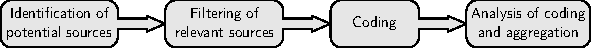
\includegraphics[width=1\textwidth]{graphics/research_process.pdf}
    \caption{Outline of the research process}
    \label{fig:researchprocess}
  \end{center}
\end{figure}

We deviated from Kitchenham's guideline on the part of data extraction. Instead
of using data extraction forms we analyzed the primary studies by coding. This
deviation was made in order to minimize how possible preconceptions would affect
the data extraction step, and to use a specialized software tool that allowed us
to record evidence in as much detail as possible.
% --> Possibility to find many different viewpoinits for the research questions
% --> Lots of items, which would have lead to much diversity in data extraction form 

\subsection{Inclusion criteria}
\label{sec:inclusioncriteria}

Based on the research questions and intended focus of the research, we defined
four facets to guide inclusion/exclusion decisions: agile software engineering,
focus on transformation, large scale, and empiricality. The first facet covers
primary studies focusing on software engineering organizations applying or
striving to apply agile methods. The second facet states that included studies
must provide insights relevant to organizational transformation, and
specifically to the research questions. The third facet underlines the
particular contribution we aim to provide with this research, namely the
exclusive focus on large organizations. The fourth facet limits inclusion to
studies presenting real world cases. These four facets were used for inclusion
and exclusion in each study selection step, including search string design,
filtering by abstracts, and full text filtering.

Table \ref{table:facets} lists the facets and gives examples on matching topics
and not relevant topics. For a study to be included it needed to be relevant
in all facets. Even if a study discussed some of the irrelevant topics it could
be included as long as it had some content matching all the facets.

\begin{table}
    \centering
    \begin{tabular}{ >{\raggedright\arraybackslash}p{0.20\textwidth}
                     >{\raggedright\arraybackslash}p{0.34\textwidth}
                     >{\raggedright\arraybackslash}p{0.33\textwidth} }
        \toprule
        Facet  &  Relevant topics  &  Not relevant topics  \\
        \midrule
        Agile software development  & 
                The organization develops software;
                The development method introduced is agile  & 
                
                Agile manufacturing;
                Scrum in management boards  \\
                
        Organizational transformation  &
                Presenting insights in the process of transformation  &
                
                Comparison of before and after;
                How agile is being used in large scale   \\
                
        Large scale    &
                At least 50 development personnel or 6 teams use agile &
                
                Scaling up from small;
                A single agile team in a large setting \\
                
        Empiricality   &
                Case studies, experience reports  &
                
                Textbooks, student experiments, theory papers  \\
        \bottomrule
    \end{tabular}
    \caption{Facets of inclusion criteria with examples of relevant and
             not relevant topics}
    \label{table:facets}
\end{table}

Examples on topics excluded by the facet of \emph{agile software development}
are agile manufacturing and applying Scrum practices in management boards, as
these do not relate to software engineering. In addition, we required that the
organizational transformation was aimed to introduce agile methods, which
excluded other development methods than agile \citep{Sagesser2013}, and use of
agile methods in other contexts than software development \citep{Hodgkins2007}.

The facet of \emph{organizational transformation} was interpreted so that the
primary study must present insights on the process of transformation. This
was the most important facet, as the pivot of this research is to examine
how the transformations happen. Examples on excluded topics are comparing the
original and agile development methods \citep{Petersen2010}, discussing use of
agile in a large organization but not describing how the new methods were
introduced \citep{Mishra2011}, and merely presenting agile tools in large-scale
use \citep{Kim2012}. These sources were excluded as they did not provide insights
on organizational transformation.
% Also [Fitzgerald 2005] on just presenting use of agile methods, no introducing

Transformation and ``scaling up'' of agile practices in use are very closely
related concepts, and in some cases they are one and the same. For instance, if
transformation begins with a pilot and spreads gradually through the
organization, the process can very well be seen as a ``scaling up'' journey.
However, we excluded cases where an initially small organization was scaled up
\citep{Maranzato2012}, and discussions focusing on processes or tools without
describing organizational change \citep{Lyon2008}.
% Also [Greening 2010] on process centered viewpoint without transformation

The facet of \emph{large scale} was interpreted as presented in section
\ref{sec:largescale}, having 50 development personnel or 6 teams as as the limit
for large scale. In some cases the source presented very vague indicators on
size. For instance, we deemed the case presented by \citet{Cloke2007} to be
included as there was indications of large-scale considerations, although the
size remained unclear. The case presented by \citet{Miller2012} was deemed to be
excluded as there was no indications whatsoever on size. A borderline exclude
was the case presented by \citet{Tudor2006} as there was no indication of issues
indicating large size, although there were several development teams.
To complicate matters, some papers talked about ``the team'' in singular when
referring to the organization \citep{Hodgkins2007}, making it clearly nontrivial
to judge whether an organization was large based on the choice of words of the
author.

Further examples on exclusion by the \emph{large scale} facet were cases with
large organizations but only a single team adopting agile \citep{Fulgham2011}.
We considered cases of single teams (although in large organizations) unrelated
to this research as our focus is on transformation of the entire organization.
Also piloting cases that resulted only in single teams using agile were excluded
\citep{Scott2008}. Finally, cases where the organization was growing to large
scale, but did not meet the size criteria at the start of the transformation,
were excluded.

% Also [Jensen 2003] with only a single team
% Possibly [Mc Cormic 2005] on single team piloting

According to the facet of \emph{empiricality} we excluded studies that did not
discuss a distinguishable real world case. We excluded textbooks, studies merely
presenting theories, and other studies that did not include any case
organization. We also excluded studies of benefits or limitations of agile in
general. Lastly, we excluded student experiments as it is implausible to
simulate the dynamics of a large organization in an experiment.


\subsection{Preliminary searches}

Before proceeding with identifying the primary studies a number of preliminary
searches were performed. The purpose of the preliminary searches was to create a
benchmark of potentially relevant papers that should be matched by the actual
search, and to evaluate different search strings. We started by examining top
ranked hits by trivial keywords that the more complex final search string might
miss. Initial searches were made using keywords that were as general as
possible, including ``agile transformation'' and ``large scale agile''.
Secondly, a trial keyword search was done in the selected databases (listed in
table \ref{table:databases}) using the following search string:

\begin{verbatim}
((agil* OR scrum OR xp OR lean) AND
(transform* OR transit* OR change OR migrat*) AND
((large AND (scale OR organization))) OR enterprise)
\end{verbatim}

From these preliminary searches we compiled a list of 117 possibly relevant
papers that the actual database search would be benchmarked against.


\subsection{Identification of primary studies}

The gathering of potential primary studies was based on a search in online
databases. The databases searched are listed in Table \ref{table:databases}. All
databases supported use of complex Boolean logic in searches, which allowed us
flexibility in constructing the search strings. The main task in the database
search was to construct a search string which yielded a reasonably large result
set. The set of matched primary studies was later amended with a small number
of studies found in references of the matched papers.

We proceeded with constructing a search string based on the facets presented in
section \ref{sec:inclusioncriteria}. However, preliminary searches had showed
that picking keywords with good precision was difficult. Especially the facet
\emph{large scale} was difficult to represent with precise words. Also the facet
of \emph{empiricality} could not sensibly be represented by keywords. We decided
to include only the facets \emph{agile software development} and
\emph{organizational transformation} in the keyword search, with the consequence
of increasing the manual filtering effort in the subsequent steps.

Having a substantial part of the matches in non-relevant areas such as agile
manufacturing, we included only articles including the term ``software'' or
articles published in relevant conferences. Instead of engineering the search
terms any further, which proved to result in excluding some relevant articles,
we chose to rely more on manual filtering. The resulting facets and keywords are
listed in Table \ref{table:searchterms}.

The database keyword search matched 1875 unique papers. The results of the
search were gathered for the selection step using reference management software.

\begin{table}[h]
    \centering
    \begin{tabular}{ l l l }
        \toprule
        Database         & URL                         & N of matches   \\
        \midrule
        IEEExplore       & http://ieeexplore.ieee.org      & 745 \\ 
        ACM              & http://dl.acm.org               & 168 \\
        Scopus           & http://www.scopus.com/home.url  & 1596 \\
        Web of Knowledge & http://apps.webofknowledge.com  & 786 \\
        \bottomrule
    \end{tabular}
    \caption{Databases included in search, and number of matched articles}
    \label{table:databases}
\end{table}

\begin{table}
    \centering
    \begin{tabular}{ >{\raggedright\arraybackslash}p{0.22\textwidth}
                     >{\raggedright\arraybackslash}p{0.70\textwidth} }
        \toprule
        Facet                  & Keywords   \\
        \midrule
        Agile methods (before \& after) &
            \texttt{agile, scrum, "extreme programming",
            waterfall, "plan-driven", RUP}\\
        Organizational transformation &
            \texttt{transform*, transiti*, migrat*, journey, adopt*, deploy, introduc*,
            "roll-out", rollout}\\
        Only software related articles &
            \texttt{(software OR (conference="agile, xp, icgse, icse"))
            AND NOT (title+abs="manufacturing" OR conference="agile manufacturing")}
        \\
        \bottomrule
    \end{tabular}
    \caption{Facets and related search terms used}
    \label{table:searchterms}
\end{table}


\subsection{Study selection}

The set of potential primary studies identified by the database search was
refined in two steps, by first filtering out abstracts and finally full text
filtering. The study selection process starting from the database search is
outlined in figure \ref{fig:selectionprocess_full}. The result of the database
search was amended with some results from the preliminary search and relevant
references from all examined papers.

\begin{figure}[b]
  \begin{center}
    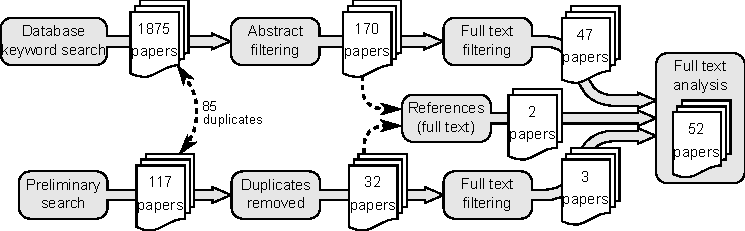
\includegraphics[width=1\textwidth]{graphics/research_process_full.pdf}
    \caption{The study selection process}
    \label{fig:selectionprocess_full}
  \end{center}
\end{figure}

The database keyword search had matched 1875 unique papers. The abstracts of
these papers were categorized independently by both Dikert and Paasivaara into
three categories: include, exclude, and uncertain. There were 1578 exclusions
and 62 inclusions that both researchers agreed on. The inclusion decisions
for the 235 abstracts with disagreement or uncertainty were resolved through
discussion. At this stage papers were excluded only if both researchers deemed
it clearly irrelevant, including any uncertain cases for full text filtering. As
a result 170 papers were selected for full text filtering.

% Inter-rater statistics
%
%                     Maria
%            excl   ???   incl    TOT
%      excl  1578    18    15    1611
% Kimi ???     84    17     8     109
%      incl    51    42    62     155
%      TOT   1713    77    85    1875
%
% ???'s =  169
% in/ex = 1706
%
% Pr(Kimi, in) = in / (tot)  =  155 / 1857 = 0.0619
% Pr(Kimi, ex) = ex / (tot)  = 1611 / 1857 = 0.8675
% Pr(Maria, in) = in / (tot) =   85 / 1857 = 0.0458
% Pr(Maria, ex) = ex / (tot) = 1713 / 1857 = 0.9225
%
% Pr(e) = Pr(Kimi, in) * Pr(Maria, in) + Pr(Kimi, ex) * Pr(Maria, ex) = 0.8031
%
% Pr(a) = (ex-ex + in-in) / tot = 0.8831
%
% k = 0.4063

Full text filtering was performed by evaluating each article against the four
facets of the inclusion criteria. Filtering was done in two steps. In the first
step Dikert extracted data relevant to the four facets. Based on the extracted
data 76 papers could be immediately deemed as included or excluded. The
remaining 94 papers were evaluated against the inclusion criteria by both Dikert
and Paasivaara, and a decision was made after discussing each paper separately.
In difficult cases Lassenius was consulted to reach a decision. As a result of
the full text filtering 47 papers were selected to be included.

We evaluated the result of the database keyword search against the benchmark
created in the preliminary search step. We concluded that 75 of the 117
preliminarily selected papers were matched by the database keyword search.
The missed 32 preliminary papers were examined, resulting in including 3
additional papers as primary sources.

In parallel with the full text filtering step the references of all papers were
also examined for relevance. Most papers used references very scarcely, typically
referencing well known descriptions of agile methods. We included 2 referenced
papers in full text analysis.

Finally, counting 47 papers from the full text filtering step, 3 papers from
preliminary searches, and 2 papers from references, 52 papers were selected
as primary studies.


\subsection{Handling of duplicate reports on a single case}

In several cases there were more than one primary study presenting the
transformation of the same organization. Duplicate descriptions of the same
organization focused typically on different aspects. For example, one paper
would highlight the viewpoint of developers \citep{Fry2007}, and another would
consider the transformation from user experience designers' point of view
\citep{Federoff2009}.

Even if the transformation of a single organization was described in many
studies, all sources that passed the inclusion criteria were included. Studies
presenting the same organization were treated as one unit so that we could gain
as much insight on each organization as possible. Conversely, there were also a
few papers that presented multiple case studies, and in those cases we treated
each studied organization individually.

As a result 42 unique organizations were identified in the primary studies. We
use the term \emph{study} to refer to the primary study publications, and the
term \emph{case} to refer to an individual case organization that may be
described in several different studies.


\subsection{Study quality assessment}

The primary research for this literature review consists almost exclusively of
industry experience reports. There were only 6 case studies with a research
method, and observations on transformation were presented only as a minor part
in these studies. Based on this finding we concluded that case studies
presenting viewpoints on organizational transformations are very scarce in
software industry. We deemed that the results would be distorted heavily and
many valuable studies would be left out if a strict quality assessment would be
part of the inclusion criteria. As a result we decided to include all experience
reports, regardless of the perceived objectivity.

The absence of research methods and subjective viewpoints of experience reports
can be seen as a factor lessening the evidence. Because of this we were
refrained from making quantitative interpretations of the data, but based the
results around describing qualitative observations. Regardless of the bias of
the primary studies, we think that the concepts that emerged from the source
material should not be questioned on a fundamental level. The overall existence
of organizational phenomena should not be questioned based on possible author
bias in experience reports.

% --> Large organizational changes are hard to measure experimentally (controlled
%     experiments?). Also due to this any student research was excluded.

% --> It may still be interesting to make some quantitative observations such as
%     a particular problem being reported in the majority of reports.

% * The primary studies did not make distinction between method, results, and
%   discussion
% 
% * The studies neither did any implications for generalizability, but rather
%   presented narratives or experiences. Some cases presented lists of
% %   recommendations.

As presented in the previous section, we allowed several descriptions of the
same case to be included. Instead of using the most complete paper as suggested
by \citet{Kitchenham2007}, we combined the results presented in each
paper and considered the case as a single unit. Keeping in mind the potential
bias caused by duplicate publications, including all papers enabled us to have a
more detailed view of the case organization.


\subsection{Coding of primary studies}
\label{sec:coding}

The primary studies were coded using the Atlas TI qualitative data analysis
software. An integrated deductive and inductive approach was chosen for coding
the primary studies \citep{Cruzes2011a}. The coding was designed to have a
contextual part and a findings part as also \citet{Cruzes2011a} suggests. A list
of codes was established for contextual information, as presented in Table
\ref{table:contextualcodes}. Codes related to the research questions were chosen
to be created by an inductive process. The reason for inducting codes rather
than using an a priori approach was to avoid the researchers' previous
assumptions of the research area to affect the choice of codes.

\begin{table}[h]
    \centering
    \begin{tabular}{ >{\raggedright\arraybackslash}p{0.26\textwidth}
                     >{\raggedright\arraybackslash}p{0.66\textwidth} }
        \toprule
        Contextual code     & Explanation   \\
        \midrule

Agile method & Agile methods used in the organization (eg. Scrum, XP) \\

Business area & The business area in which the organization operates. \\

Organization size & Mentioning the size of the case organization. \\

Time of transformation & When the transformation has been in
progress, or how long the transformation has taken. Possibly relative to
the time of the research. \\

Research process & The paper describes a research process. \\

Geographical location & Where the organization is located. \\

Large scale definition & A definition of large-scale software development. \\

Multisite / GSD & Mentioning of a multisite organization. \\

        \bottomrule
    \end{tabular}
    \caption{Context information specified to be gathered from primary studies.}
    \label{table:contextualcodes}
\end{table}

To give direction for code induction, seven different code families were
established on beforehand, as presented in Table \ref{table:codefamilies}. A
description defining scope and examples for codes were defined for each family.
The example codes would not necessarily be used as actual codes, and would not
represent the entire or final scope of the families.

The inductive coding was done according to the guidelines described below.

A passage of text that presents any concept relating to the research questions
or the contextual codes becomes a quotation. If the quotation corresponds
closely to a concept that has already been coded the existing code is used.
Otherwise a new code is created, and the code is assigned to one of the
predefined code families. The labels of existing codes may need to be adjusted
when new quotations are assigned. A clarifying description is written for every
code, so that the precise meaning of the codes can be reviewed. Many codes may
be assigned to one quotation and quotations of different codes may be
overlapping.

The length of the text passage that make up a quotation may vary. For the
contextual codes the quoted passage should be of minimal length. For other
quotes the length of the quotation should be long enough to highlight the
context of the concept the quotation, varying from a few sentences to one
paragraph, or even several paragraphs. As an example of context of the
quotation, if a transformation challenge is described by a quotation it would be
good if also the source or resolution of the challenge could be included in the
quoted text passage. Having enough context should broaden the understanding
of the coded concept when looking at the quotation in isolation.

% -- Considering that mentioning the inclusion of a factor as a success, then
%    would the absence of the same factor be a challenge?

\begin{table}
    \centering
    \begin{tabular}{ >{\raggedright\arraybackslash}p{0.31\textwidth}
                     >{\raggedright\arraybackslash}p{0.61\textwidth} }
        \toprule
        Code family          &  Description
        \\
        \midrule

        RQ1: Reason to change &
        Reasons to start the transformation (demand for faster delivery). \\

        RQ2: Transformation process &
        Statements that describe the transformation process (top-down, big bang,
        step wise). \\

        RQ3: Challenges &
        Statements that present challenges in the transformation (change resistance).
        \\

        RQ3: Success factors &
        Statements that present success factors in the transformation (management
        support).
        \\

        Investing in change  &
        Factors that present how the organization is investing in the
        transformation (training, consultants, tools). \\

        Practices &
        Distinguishable practices that are used or established during transformation.
        Factors presented as neutral relating to successes and challenges.
        (coaching, piloting, continuous integration, communities of practice) \\
        
        Contextual &
        Contextual codes defined in Table \ref{table:contextualcodes}. \\
        
        \bottomrule
    \end{tabular}
    \caption{Code families defined before start of coding. Examples on
    potential codes to be inducted in parentheses.}
    \label{table:codefamilies}
\end{table}

\begin{table}
    \centering
    \begin{tabular}{ l r r }
        \toprule
        Code family    &  Codes  &  Quotations
        \\
        \midrule
        RQ1: Reason to change &        30 &  123 \\
        RQ2: Transformation process &  16 &  580 \\
        RQ3: Challenges &              40 &  323 \\
        RQ3: Success factors &         44 &  260 \\
        Investing in change  &          5 &  137 \\
        Practices &                    11 &  170 \\
        Contextual &                    8 &  215 \\
        Total &                       154 & 1575 \\
        \bottomrule
    \end{tabular}
    \caption{Number of codes and quotations per code family, as the final result
    of coding the primary studies}
    \label{table:codecount}
\end{table}

\clearpage

The total number of codes and quotations created in the coding process is
presented in Table \ref{table:codecount}. The total number of quotations is less
than the sum of quotations in the categories because a single quotation may have
multiple codes.

\subsection{Validation of coding}

Coding was done by only one researcher due to resource constraints and volume of
source material. As recommended by \citet{Kitchenham2007} we conducted
an experiment with the goal to assess the consistency of coding that two
independent researchers may achieve.
In the experiment Dikert and Paasivaara coded independently a sample of five
primary studies. The sample was hand picked as a representative subset of the
source material. The coding was done relying solely on the guidelines presented
in the previous chapter, and the researchers were careful not to discuss the
choice of codes or interpretations relating to codes before the experiment was
completed. Finally the independent codings of the two researchers were analyzed
with two metrics: by the number of matching themes found, and by the amount of
overlap in quotations similar codes have.
% See Kitcenham, chapter 6.4

The metric of matching themes measures how well the independent researchers are
able to induct similar codes from the source material. As codes are inducted it
is likely that two researchers label similar quotes differently. To overcome
this problem we defined higher level themes under which the individual codes
were organized. Through discussion we made decisions on whether differently
labeled codes could be organized under the same theme or not. Table
\ref{table:codingexperiment} presents the total number of themes the researchers
found in each document, and how many of the themes were matching. We concluded
that on average two of three themes found by one researcher were similarly found
by the other researcher, but one of three themes was not found by the other
researcher.

The metric of quotation overlap measures how well the quotations for similar
codes match between two independent researchers. The intent is to measure how
well codes that are deemed similar by their names match in the actual quoted
text. We assigned a quotation overlap score for each code in themes that both
researchers had found. A score of 3 was given for matching codes whose quotation
content was virtually the same for both researchers. A score of 2 was given if
the quotations were mostly the same, but other researcher had included one text
passage that the other had missed. A score of 1 was given if roughly half of the
quotation was the same. If the quotations had less similarity than this a score
of 0 was given. One code provided typically 1 to 3 quotations per document. The
quotation overlap score was counted including only codes that had matching
themes. We concluded that the average quotation overlap score was 2.2.

\begin{table}
    \centering
    \begin{tabular}{ l r r r }
        \toprule
        Document    &  Matching themes  &  Total themes  &  Quotation overlap (0-3) \\
        \midrule
        P1          &  14  &  19   &  2.1  \\
        P2          &   6  &  11   &  2.4  \\
        P3          &   7  &  11   &  2.1  \\
        P4          &   2  &   4   &  2.3  \\
        P5          &  12  &  16   &  2.0  \\
        \bottomrule
    \end{tabular}
    \caption{Result of independent coding experiment}
    \label{table:codingexperiment}
\end{table}

Combining the quotation overlap result and the result that inductive coding
yielded similar themes with a factor of two thirds, we conclude that two
different researchers should agree completely on at least half of the quotations
in the source material of our study. This agreement includes both that the
researchers select the same text passage as a quotation, and that researchers
agree with the meaning of the quotation. Further interpretation of the
quotations and codes will still remain a subjective matter.


\subsection{Synthesis of primary studies based on coding}

The synthesis of findings was created based on the result of coding presented in
section \ref{sec:coding}. An initial organization of codes into categories was
made based on the labels of the codes. Each codes was linked to a single
research question, so the categorization of codes was made separately within
the topic of each research question. The categories of codes were labeled
appropriately to give a high level description of the linked codes. Some codes
having minor importance and few quotations were left out.

After assigning each code to a unique category, the content of the categories
was studied. Each category was studied by reading through each quotation of each
code included. Typically the quotations were displayed and examined in their
original context, considering also surrounding paragraphs of the quotation.
Notes were made on each quotation presenting noteworthy observations. Based on
the notes, an accurate description emerged for each code.

As an accurate description had been created for each code, the initially defined
categories could be refined. Some codes were re-categorized, and the definitions
of a few categories were revisited, until a final ordering was reached. The
results are presented according to the final categorization.

% * If a code had more quotations there were more observations made (longer
%   result text)


% ---------------------------------------------------------------------
\clearpage

\chapter{Results}
\label{sec:results}

This section presents the findings of the literature review. In the first
subsection a meta analysis of the analyzed papers is presented. In the
subsequent sections findings are presented organized according to the research
questions.

The methods used for extracting the results were described in section
\ref{sec:method}. Note that the term \emph{study} is used when referring to a
primary study publication, and the term \emph{case} is used when referring to an
organization which may be described in several studies.

\section{Overview of primary studies}

The results of this study include findings from 52 primary studies presenting
how 42 different large software organizations introduce agile methods. Most of
the included studies were experience reports (45 studies), and in many cases it
was evident that the author had been personally involved in the transformation.
Only 6 of the included studies had a research method explicitly stated. One of
the studies was an interview article. The publication forums of the primary
studies were distributed so that 47 sources were conference proceedings, 4
sources were journal articles, and one source was a technical report.

Figure \ref{fig:transformation_time} summarizes the publication years of the
primary studies, and the years when the transformations were reported to have
started. All studies and transformations were dated after year 2000. There were
peaks in transformation studies in years 2008 and 2011. The studies were
typically published two years after the start of the transformation.

\begin{figure}[b]
  \begin{center}
    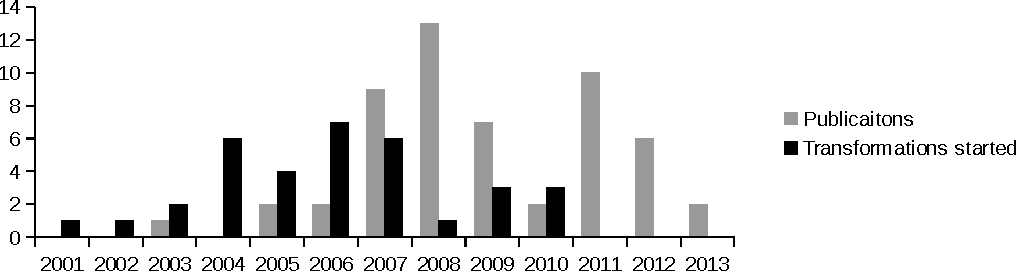
\includegraphics[width=1\textwidth]{graphics/transformation_time.pdf}
    \caption{Publication years and reported start years of transformations}
    \label{fig:transformation_time}
  \end{center}
\end{figure}

The size of the organizations varied from the minimum included size of 50 to
18,000 people. The median size was 300 people. In 7 studies the size was
presented in terms of teams, ranging from the minimum of 6 teams to 150 teams.
The median was 10 teams. In 8 studies there was no direct indication on size
but the issues discussed revealed that the organization was of large size
according to our definition. The distribution of organization sizes is presented
in figure \ref{fig:organization_size}.

\begin{figure}[!t]
  \begin{center}
    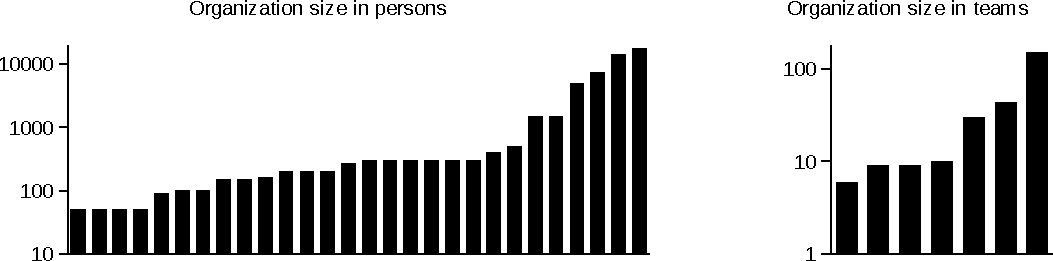
\includegraphics[width=1\textwidth]{graphics/organization_size.pdf}
    \caption{Distribution of organization sizes in primary studies}
    \label{fig:organization_size}
  \end{center}
\end{figure}

\begin{table}[!t]
    \centering
    \begin{tabular}{ l r }
        \toprule
        Business area    &  Case organizations   \\
        \midrule
		Online services for consumers and business  &  9  \\
		Telecommunications                          &  7  \\
		Enterprise management                       &  5  \\
		Banking and financial services              &  4  \\
		Health care                                  &  3  \\
		IT services                                 &  2  \\
		Government                                  &  1  \\
		Information security                        &  1  \\
		Not specified                               & 10  \\
        \midrule
		Total                                       & 42  \\
        \bottomrule
    \end{tabular}
    \caption{Business areas of case organizations in primary studies}
    \label{table:businessareas}
\end{table}

The business areas of the case organizations are presented in table
\ref{table:businessareas}. Different business areas were represented somewhat
evenly. Online services was the largest group, including companies
providing software as a service solutions for businesses, online media players
for consumers, online services for consumers, and communication software for
businesses. The second largest group was telecommunications, including companies
such as British Telecom, Cisco, Ericsson, and Nokia Siemens Networks. The third
largest group was enterprise management solution providers with products for
business process management, project portfolio management, and facility
management.


\section{Agile methods used}

The agile methods reported being used in the transformed organizations are
summarized in table \ref{table:agilemethods}. The most prevalent method was
Scrum, which was the sole agile method mentioned in 25 cases. The second most
mentioned agile method was Extreme Programming (XP). Lean software development
was mentioned in some studies, although combined to Scrum in all cases. Other
agile methods mentioned were Unified Process, ADM, and Rapid Application
Development. In one case the agile method was not named.

It was quite common that organizations sought to combine agile methods.
Especially Scrum, XP, and Lean software development were used together. In
addition, many cases mentioned use of XP practices without explicitly stating XP
as the process being used (such as test driven development and continuous
integration). Combining and customizing agile practices was also evident in that
many organizations viewed the agile method as continuously evolving.
Organizations evolved the agile methods for instance through retrospectives and
continuous improvement.

\begin{table}[h]
    \centering
    \begin{tabular}{ l r }
        \toprule
        Method                             &  N  \\
        \midrule
        Scrum                              &  25 \\
        XP                                 &  4  \\
        Scrum and XP                       &  5  \\
        Other                              &  4  \\
        Combining Lean to an agile method  &  6  \\
        Not specified                      &  1  \\
        \bottomrule
    \end{tabular}
    \caption{Agile methods reported in number of cases}
    \label{table:agilemethods}
\end{table}


\clearpage

\section{Reasons to change}

As stated by Research Question 1 we investigated the reasons organizations start
a transformation process towards agile software development. Most primary
studies mentioned reasons for starting the transformation, and only 7 cases of
42 did not mention any reasons. In the cases giving no specific reason to change
it was simply mentioned that management had decided to change the organization.
The reported reasons for starting an organizational change towards agile are
summarized in figure \ref{fig:reasonstochange_summary}.

% Some cases reported that the organization had been successful in waterfall
% delivery for a long time before the agile transformation.


The most prominent reason to start the transformation was that business demanded
shorter lead times and faster delivery. Other top reasons to start change were
dysfunction in management, overhead in the current process, problems in
scheduling, and demand to improve quality.


\begin{figure}[h]
  \begin{center}
    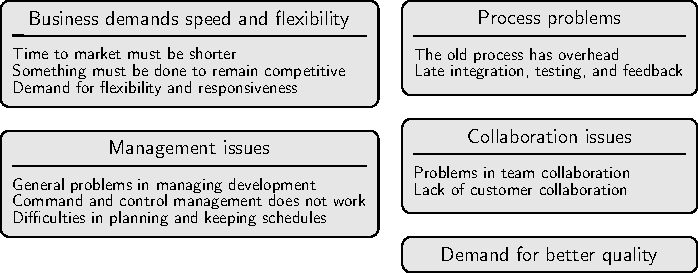
\includegraphics{graphics/reasonstochange_summary.pdf}
    \caption{Reasons why the studied organizations started an agile
             transformation}
    \label{fig:reasonstochange_summary}
  \end{center}
\end{figure}

\subsection{Business demands speed and flexibility}

Most cases reported that a major reason to change was that business demanded
improvement. Most companies wanted to improve their competitiveness, or even
feared that they are losing competition. The way to respond was to improve
delivery speed and responsiveness to change. Table
\ref{table:reasonstochange_business} presents business related reasons to
introduce an agile model.

\begin{table}
    \centering
    \begin{tabular}{ >{\raggedright\arraybackslash}p{0.51\textwidth}
                     >{\raggedright\arraybackslash}p{0.41\textwidth} }
        \toprule
        Business reasons for starting a change   &  Described in  \\
        \midrule
        Time to market must be reduced    &  P17, P18, P32, P38, P39, P47  \\
        Delivery is considered slow       &  P2, P8, P25, P36, P46, P49  \\
        Something must be done to remain competitive  &
                P9, P10, P11, P18, P19, P32, P38, P42, P49  \\
        Business partners demand faster delivery  &  P5, P23, P39, P40, P46  \\
        Need to accommodate change during projects  &
                P4, P8, P18, P25, P26, P33, P36, P39, P42, P49, P51, P52  \\
        \bottomrule
    \end{tabular}
    \caption{Business related reasons for starting an agile transformation}
    \label{table:reasonstochange_business}
\end{table}

The most frequently mentioned reason for introducing agile methods was the demand to
deliver software faster and more frequently. A common statement was that it was
necessary to reduce the time to market (TTM) [P17, P18, P32, P39, P47]. As
stated in one study: ``The market was moving faster than the development group
was able to deliver'' [P38]. Long cycle time, i.e. time from start of project to
delivery, was seen as a problem in itself [P25, P36]. Some studies indicated
that the organizations set as one of the transformation goals to deliver
software faster [P2, P8]. Other cases described that development was generally
considered as slow [P36, P46, P49].

Commercial competition and market situation was seen as a trigger for
transformation. Especially speed of delivery was seen as a means to respond to
the competition [P9, P38]. As Greening [P19] describes: ``The average release
duration peaked at 41 and 35 months, an alarming state that could enable
competitors to gain market share.''. In many cases the transformation was seen
as essential for the company to remain competitive [P10, P11, P18, P42, P49].
For instance, British Telecom realized that ``From a strategic view, there is
little alternative than to change the old ways of working'' [P32].

Demands for change and improvement were also expressed by internal and external
customers. Again, the requests of the customers reflected the need of faster
development and release cycles [P5, P39]. As described in one study: ``Speed of
delivery is of the essence -- customers are no longer prepared to wait for 18
months or more for solutions to be delivered'' [P23]. In some cases business
partners expressed mistrust in the original way of conducting development [P40,
P46].

Yet another factor pushing for improvement was the need to accommodate change
during development. Organizations saw agile as an opportunity to improve
responsiveness to change in general [P25, P26, P42].
Some organizations faced difficulties when changes to plans were needed. For
instance, the organizational structure made adapting to changes difficult [P52],
and making changes created management overhead [P51]. Other organizations saw an
business advantage in enabling priorities to be changed as required [P8, P39].
Domain knowledge will deepen during projects and environments will inevitably
change, and therefore the requirements should not stay fixed [P4].
Customers and business representatives were in many cases attributed as the
sources of change requests, and the responsiveness to customer requests needed
to be improved [P18, P33, P36, P49].

\subsection{Management issues}

The way software development was managed was typically seen as problematic. The
problems related to project management, people management, and managing
schedules. Management related problems that the transformation was hoped to
correct are listed in table \ref{table:reasonstochange_management}.

\begin{table}[b]
    \centering
    \begin{tabular}{ >{\raggedright\arraybackslash}p{0.51\textwidth}
                     >{\raggedright\arraybackslash}p{0.41\textwidth} }
        \toprule
        Management problems           &  Described in  \\
        \midrule
        Software development is managed badly   &  P8, P21, P30, P38, P44, P49  \\
        Command and control style management    &  P9, P25, P30, P40, P44  \\
        Scheduling and estimation is difficult  &  P16, P19, P21, P30, P33, P40, P41, P51  \\
        \bottomrule
    \end{tabular}
    \caption{Management problems stated as reasons for organizational change}
    \label{table:reasonstochange_management}
\end{table}

In many organizations the project management practice was in a state of
dysfunction, and it needed to be corrected. Project management problems included
constantly recurring crisis events [P30], managers ignoring prioritization of
tasks [P38], and reluctance towards focusing on delivering business value [P49].
Some cases stated that projects simply failed [P21]. Some organizations wanted
to improve generic project management practice, such as risk management [P8],
management of offshoring [P38], and generally improving the quality of life of
team members [P44].

Command and control style management where ``a few people, usually those
farthest from the action, made the decisions without directly involving the
developers doing the actual work'' was highlighted as a problem [P44]. For
instance, schedules could be dictated by management, and teams had to comply to
them regardless of the workload [P9]. As a result teams were overworked and
needed stretch far to finish projects on time. Low morale and motivation were
identified as problems that needed to be fixed, and agile was seen as a solution
[P25, P30, P40].

Yet another problem in managing development was problems with schedules.
Some cases described schedules as unpredictable and estimation being difficult
[P16, P30, P40, P51]. In other cases it was reported that release deadlines were
often missed [P19, P21, P33, P41].

\subsection{Process problems}

The old way of working was acknowledged to have problems which needed to be
corrected. A summary of weaknesses in the original process is presented in table
\ref{table:reasonstochange_process}.

\begin{table}[b]
    \centering
    \begin{tabular}{ >{\raggedright\arraybackslash}p{0.51\textwidth}
                     >{\raggedright\arraybackslash}p{0.41\textwidth} }
        \toprule
        Problems in the old process           &  Described in  \\
        \midrule
        Excess and overhead in process     &  P9, P24, P35, P36, P38, P40, P46, P49, P51  \\
        The process is being ignored       &  P6, P9, P46, P49  \\
        Late integration, testing, and feedback  &  P5, P25, P33, P40, P50  \\
        New practices can not be integrated in the old process  &  P10, P26  \\
        The old process does not scale up  &  P16, P30, P50, P51  \\
        \bottomrule
    \end{tabular}
    \caption{Problems because of which the old process should be changed}
    \label{table:reasonstochange_process}
\end{table}

A most typical known problem was overhead in process, which showed as bureaucracy and
needless costs. Examples on overhead in process were unproductive meetings
[P38], sign-offs and gates [P9], excessive focus on conformance to process
[P40], and change management overhead [P51]. Creating excessive documentation
instead of business value was seen as a problem in some cases [P24, P35]. From
business representatives point of view the processes were unreasonably costly,
while at the same time insufficiently capable of delivering business value [P36,
P46, P49]. In one case business realized that customers did not see any benefit
in the heavy CMMI based process [P24].

A heavy process resulted often in ignoring the process, only paying ``lip
service'' to the process, or applying its steps retroactively [P6, P9, P49].
Seffernick [P46] describes how applying the waterfall process had teams ``still
developing the same old way but slower because of the additional process''.

A slow process with long cycle times leading to late feedback was a problem in
the old model. A large investment was required before results were visible [P5],
and there was variances in expectations and what was delivered [P40]. A related
problem was late integration which caused extra work [P25]. As organizations
grew and products became more complex test cycles began to lengthen, which
hindered flexibility and reduced speed [P33, P50].

A few organizations were experiencing rise of agile methods at grass roots
level, but the agile teams could not integrate efficiently with other parts of
a waterfall organization. Tensions arose when teams using different development
approaches attempted to work together on products [P10]. On a team level agile
had enabled some flexibility, but that flexibility could not be leveraged on the
scale of the entire organization [P26].
This kind of experiences drove the organization to deploy agile on a full scale.

Still one problem was that some growing organizations experienced that the old
development method did not scale up [P16, P30, P50, P51].


\subsection{Other reasons to change}

There were still a number of problems that were given as reasons to change.
In addition to the above mentioned problems, organizations were striving for
better collaboration and quality. Table \ref{table:reasonstochange_other} lists
other issues that drove organizations to change.

\begin{table}[b]
    \centering
    \begin{tabular}{ >{\raggedright\arraybackslash}p{0.61\textwidth}
                     >{\raggedright\arraybackslash}p{0.31\textwidth} }
        \toprule
        Reasons to change           &  Described in  \\
        \midrule
        Teams can not collaborate properly   &  P21, P38  \\
        Silos and internal boundaries in organization   &  P27, P40, P46  \\
        Lack of customer collaboration       &  P4, P26, P40  \\
        Demand for better quality            &  P2, P4, P25, P31, P30, P38, P41, P42  \\
        \bottomrule
    \end{tabular}
    \caption{Other reasons why organizations wanted to change the way of working}
    \label{table:reasonstochange_other}
\end{table}

Many organizations experienced problems in communication and collaboration
between projects, teams, and even members of a single team [P38, P21].
Teams were in many cases organized around components and were working in silos.
Working in silos diluted focus and made adapting to change difficult, as teams
could only focus on their limited area of expertise [P7]. Functional silos acted
against creating a shared purpose in operating [P40], and resulted in a ``ball
over the wall'' mentality [P46]. Distance between teams was also created by
document driven communication, and was causing misunderstanding of requirements
[P24].

Too little customer and user collaboration led to problems in some
organizations. For instance, too late user involvement led to change requests
late in the project [P40]. There was a wish to collaborate more frequently and
in less formal ways [P4, P26].

% There was also a desire to improve team motivation and commitment, and
% collaboration between management and developers [P39].

% Examples of problems with requirements was too much focus on the documenting
% aspect instead of providing understanding [P24, P49], and ignoring the fact that
% requirements and understanding are evolving during a project [P4].
% 
% In some cases the organization of work and management was such that it caused
% lack of focus the development [P7], and prioritization of what to work on was
% not done efficiently [P38, P39].

Lastly, the original model was seen as a cause for quality problems.
Several studies mentioned a demand for better quality, and quality improvement
was set as a goal for the agile transformation [P25, P31, P41, P42]. New feature
development was being prioritized over bugfixes, and technical debt was
developing [P30, P38]. Improvement in external quality and customer satisfaction
were anticipated from agile development [P2, P4].


\clearpage

\section{Transformation process}

The second research question was aimed to discover how the process of
transformation can be described.
We provide an answer to Research Question 2 in several parts. First the initial
states of organizations are described. Secondly, we present a model for
categorizing transformation types. In the rest of this section we discuss
typical arrangements that relate to the change process, including how training
and piloting is arranged, how change is lead, and what investments are done.

The fact that every organization is unique creates challenges in giving generic
descriptions on how transformations proceed. Further, publications tended to
provide more focused viewpoints rather than describing the transformation
process itself. Therefore it was not sensible to attempt constructing a detailed
model on how large organizations adopt agile methods.
Table \ref{table:transformation_descriptiontypes} presents types of insights
each primary source provided in relation to Research Question 2.

\begin{table}[h]
    \centering
    \begin{tabular}{ >{\raggedright\arraybackslash}p{0.52\textwidth}
                     >{\raggedright\arraybackslash}p{0.40\textwidth} }
        \toprule
        How transformation is described   &  Primary sources  \\
        \midrule
        Narrative description of transformation process &
                P3, P5, P6, P9, P11, P12, P16, P18,
                P24, P27, P30, P36, P40, P41, P46   \\
        Application of agile methods seen from a specific viewpoint (e.g. coaching team) &
                P10, P13, P15, P19, P23, P32, P34,
                P39, P47, P48, P50, P52    \\
        Viewpoints of challenges and success factors  &
                P17, P20, P21, P29, P37, P38, P49   \\
        Discussion on establishing large scale agile practices  &
                P7, P8, P31, P42, P43, P44, P45   \\
        Only brief discussion on transformation process  &
                P1, P2, P4, P14, P22, P25, P26, P28, P33, P35, P51  \\
        \bottomrule
    \end{tabular}
    \caption{The theme of each primary source, in relation to providing
             insights of the transformation process}
    \label{table:transformation_descriptiontypes}
\end{table}


\subsection{The initial state of the organization}

We investigated the initial state of the case organizations before the
transformation. The typical initial process model was described as waterfall, as
stated in 25 cases. In several cases the authors characterized the initial state
of the organization as ``traditional''. CMMI was presented as a driver for the
original process in 4 cases. Other process models the studies named were RUP
[P19], Prince2 [P51], and Macroscope [P14]. In 9 cases the initial state was not
described.

The old model was described in most cases briefly and in a neutral sentiment.
Waterfall development in general was referred to as ``traditional, plan-based
methods'' [P25], ``traditional phase-based approach'' [P36], or ``old fashioned
process driven waterfall'' [P23]. Korhonen [P25] referred to the model presented
by \citet{Royce1970} when describing the initial state.

In some cases specifics of the old model was criticized. The characteristics of
the old process models were described as having ``many gates and sign-offs
required by upper levels of management'' [P9], ``lot of bureaucracy in project
management and a strict hierarchy of requirements communication'' [P39], and
``project managers typically used a command-and-control philosophy'' [P44].

In a few cases the initial process model was less rigid, and closer to the agile
model that was to be introduced. Examples of such loose process models were
described: ``The choice of development methodology is one of any number of
degrees of freedom granted to teams at Amazon. Development teams are expected to
solve their problems in the best way possible'' [P3], ``the R\&D group leveraged
a loose, waterfall-based process with an entrepreneurial culture'' [P16]. Some
organizations had even signs of agile development on team level although the
surrounding organization operated in a waterfall fashion. This was described as
``Agile and Scrum were increasingly popular and emerging at a grass-roots level,
at a corporate level Yahoo! still embraced a more traditional product
development process'' [P10], and ``some teams had applied scrum on the team
level, despite the surrounding organization that was working with a waterfall
software engineering model'' [P26].

In a few cases the organization initially lacked strict process. For instance
Long [P30] describes the initial state in the following way: ``Project scope was
in constant flux. Well-meaning market and product owners routinely inserted new
requirements during product development.''.

Some authors describe development being originally organized in silos. For
instance, Ranganath [P40] describes that ``Teams operated in silos.
Collaboration, shared purpose and ownership for outcomes were hard to find''.


\subsection{Modes of transformation}

Based on the primary studies we identified two dimensions in the characteristics
of transformation processes. The first dimension is the pivot point of
leadership in change. This dimension has two extremes: top-down leadership where
the change is mandated by management, and bottom-up leadership where the change
emerges from team level. The second dimension is the velocity of the change.
Organizations were reported to perform transformations as a big bang or
overnight fashion, or as a step wise process lasting for a long time. Figure
\ref{fig:transformation_dimensions} summarizes the transformation process
dimensions.

\begin{figure}[h]
  \begin{center}
    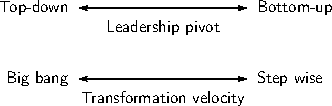
\includegraphics{graphics/transformation_dimensions.pdf}
    \caption{Dimensions for categorizing transformation types}
    \label{fig:transformation_dimensions}
  \end{center}
\end{figure}

We do not quantitatively measure cases on the transformation process dimensions,
because the criteria for creating a measurement would be vague. For instance, we
do not think that presenting a single quantitative measurement of the weight
point of leadership on an axis between management centric and team centric would
describe reality accurately. The dimensions of pivot of leadership and
transformation velocity nevertheless exist.

As the primary sources describe, transformation cases combined the dimensions of
leadership pivot and velocity. Four combinations of the characteristics could be
observed. Figure \ref{fig:transformation_types} summarizes the combinations of
transformation characteristics.

\begin{figure}[h]
  \begin{center}
    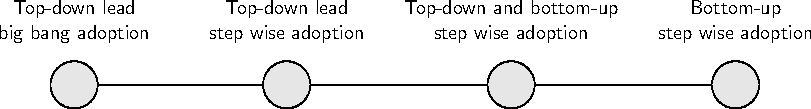
\includegraphics[width=1\textwidth]{graphics/transformation_process.pdf}
    \caption{Categorization of transformation types}
    \label{fig:transformation_types}
  \end{center}
\end{figure}

The most extreme case of adoption was a big bang transformation. To realize such
a large change it is necessary that the change was centrally coordinated.
For step wise transformations the the amount of management and development team
involvement varied. At one extreme, the change was lead by management while
teams played a passive role. At the other end management was described to be
reluctant to change while teams pushed for change. Many cases took a middle
course where both management and development dealt with the transformation on
their respective level of influence.

As a concept separate from the dimensions of leadership pivot and velocity, the
transformation was described as a continuous process. There were a few
viewpoints illustrating the concept of continuous transformation. Several
organizations were striving to introduce a culture of continuous improvement,
which would make organizational adjustment a permanent state. In many cases the
agile transformation was not considered to have ended at any distinct point in
time, and the impression that it was still ongoing was given. Finally,
transformation was simply described as hard work that will inevitably take a
long time.


% Mentioning big bang versus step wise [P16].



% %%%%%%%%%%%%%%%%%%%%%%%%%%



% ---------------------------------------------------------------------



% ---------------------------------------------------------------------




\subsection{How change was lead}

A significant change effort requires entities in the organization who take
leadership in the change. Getting a large group of people aligned towards a
common goal, in many cases a completely new way of working, requires that
someone takes charge for the undertaking. The primary sources showed evidence of
leadership for change on all organizational levels. Table
\ref{table:transformation_leadership} summarizes different types of change
leaders that were discovered.

\begin{table}[h]
    \centering
    \begin{tabular}{ >{\raggedright\arraybackslash}p{0.51\textwidth}
                     >{\raggedright\arraybackslash}p{0.41\textwidth} }
        \toprule
        Change leaders         &  Described in  \\
        \midrule
        High-up change leaders or sponsors  &
                P3, P5, P24, P31, P36, P38, P46, P49  \\
        Agile task group for coordinating change   &
                P4, P16, P18, P21, P23, P25, P30, P40, P41,
                P43, P45, P48, P49, P50  \\
        Change leaders on development team levels  &
                P2, P6, P9, P14, P17, P18, P27  \\
        Informal spreading of agile awareness  &
                P3, P6, P14, P40  \\
        \bottomrule
    \end{tabular}
    \caption{Summary of entities leading change in the agile transformation}
    \label{table:transformation_leadership}
\end{table}


% High-up change leaders

In many cases it was described that the change was initiated by a limited number
of people in high-up positions. In these cases typical positions attributed for
giving the initial push for change were CxO's, vice presidents, and directors.
In these cases it was highlighted that one or very few high-up persons affected
significantly the start or expansion of the agile transformation. In some cases
the change leader was a new hire [P5, P38, P46].

The presence of a high-up manager was described to underline the organization's
commitment for change when dealing with employees or other stakeholders [P24].
The firm commitment of the high-up leader was key in keeping the agile
transformation on course in cases where objections or other problems arose [P5,
P14, P36, P46]. Another important role of the change leader was to persuade and
work for getting other people raise an interest in agile methods [P3, P31, P38,
P46, P49].

% Agile task force

Many organizations formed an agile task force or similar entity for coordinating
and leading the change. It was typical that in the beginning of the
transformation, or when it had been acknowledged that the old model had
problems, a work group was founded for coordinating the changes to be done. The
change team usually consisted of management personnel [P43, P50], and was
reinforced with external agile consultants [P18, P21, P25, P30]. Some cases
highlighted that the team had a cross organizational staff who were familiar
with the varying functions that would be affected by changes [P4, P16, P21, P41,
P48]. It was important that there was a group of people who were strongly
committed to making a change happen [P43].

The typical first task of the change team was to decide on an alternative
delivery method to solve problems in the old model [P21, P30]. During the
transformation the team stimulated agile adoption in the organization [P18, P45,
P49]. Other examples on the change team's tasks were informing people on the
agile model [P4], educating and coaching [P16, P45, P48, P49], creating an agile
cookbook [P23], and organizing presentations and workshops [P25, P41]. The
change team also assessed the success of transformed teams, and worked for
repeating their success across the organization [P16, P40, P41]. The change team
was empowered to act on removing impediments they discovered [P16, P50].

% Other change leaders

Beyond executive positions, leadership for change emerged also on lower
organizational levels. In many cases these change leaders were still in
management positions [P14, P18, P17]. There were also agile champions in teams
who drove the change on a grassroots level [P6, P9, P27].
As with higher-ups, these people worked for making agile methods familiar [P2,
P6, P9, P17], making change stick [P2, P18], and persuaded others to use agile
methods [P2, P9, P14].
Benefield [P6] describes that people in teams were well able to adjust the
application of the agile process as they were familiar with the problems at
hands. It was however hard to find people who both understood the agile
principles well, and knew how to coach within the team [P6].
% Also coaches in [P2], and a team in [P16]

Chung and Drummond [P9] give a further description of grassroots level
leadership. Yahoo! initially used a team of coaches to help applying agile, but
the coach team failed to make agile take root. The coaches were later disbanded
due to reductions in budget. The agile practitioners in teams took over the
leadership for the continued application of agile [P9].

% Informal spreading of awareness

Change leadership showed on the lowest level as informal spreading of awareness
of agile methods.
Benefield [P6] describes that the strongest force over other change leaders was
letting agile knowledge spread virally. New Scrum teams were emerging as people
heard of the new methodology [P6]. In some cases interest groups were used to
stimulate viral spreading of agile [P14].
It was similarly described that in an organization with an introverted culture
the proclamations of managers could not match with the power of practitioners
explaining to others how they had succeeded in with the agile method [P40].
Even casual hallway talks could spread the word effectively, and it was also
easier to encounter people from other parts of the organization in an informal
context [P3].


\subsection{Training, coaching, and awareness}

During transformation periods organizations invested in activities aimed to
incorporate the new model into the thinking of people. People were new to agile
methods, and a common understanding needed to be created. Training, coaching,
and public events were used for communicating the new model to a significant
part of the organization. Describing the use of training and coaching was a very
prominent facet in transformation cases.
Table \ref{table:transformation_training} summarizes activities that
organizations use for deepening the understanding and awareness of the new
development process being applied.

\begin{table}[h]
    \centering
    \begin{tabular}{ >{\raggedright\arraybackslash}p{0.31\textwidth}
                     >{\raggedright\arraybackslash}p{0.61\textwidth} }
        \toprule
        Activity           &  Described in  \\
        \midrule
        Training    &
                P3, P6, P8, P9, P11, P16, P18-P21, P23-P25, P27, P30,
                P32, P35, P37, P39-P41, P43-P46, P48-P51  \\  % 29
        Coaching    &
                P1-P3, P6, P8, P9, P11, P16, P18, P23, P27, P29,
                P31-P33, P36, P39-P41, P45-P47, P49, P50, P52  \\  % 25
%         In-house coaching   &
%                 P1-P3, P6, P11, P16, P23, P29, P31, P32,
%                 P39, P41, P45, P47, P49, P50, P52  \\    % 17
        Seminars and workshops   &
                P1-P4, P7, P9, P10, P18, P11, P16, P23, P25,
                P26, P27, P32, P41, P44, P46, P47   \\   % 19
        Communities, special interest groups  &
                P3, P6, P7, P9, P10, P11, P12, P14, P32, P41,
                P42, P45, P47, P52  \\   % 14 
        \bottomrule
    \end{tabular}
    \caption{Summary of activities for building awareness and knowledgeability
             in the agile way of working}
    \label{table:transformation_training}
\end{table}


% Training

As the organization is changing it is necessary to train people so they get
familiarity with the new model that is being pursued. The majority of cases
described the use of training in the transformation.
Most typically the change leaders and pilot teams were the first to attend
formal training on agile development. Management was also usually among the
first ones to receive agile training. In some cases particularly management
received more in-depth training [P11, P16, P24]. In addition to providing an initial
understanding of agile it was considered important that the key people get a
common understanding of the method [P11, P24, P39].

After key people had attained knowledge on agile, and pilot teams had possibly
tested the methods, other teams received training on the new development model.
In some cases the training of development teams was described to be brief [P11,
P16, P20]. Other cases implemented a full day workshop [P18, P23, P32, P41,
P45], and some organizations invested even in multi-day training [P9, P19, P37,
P49].
The reduced training for engineers was compensated with coaching during ongoing
projects [P11].

Several cases mentioned that the first introductory events were held by known
industry experts [P3, P19, P25, P27, P30, P46]. External consultants were also
often used as trainers [P18, P25, P40, P41, P49, P51]. In some cases a limited
number of people with agile knowledge was first trained or acquired, and later
the training was arranged with internal resources [P3, P11, P24, P25, P41, P46,
P49, P51].
The training curriculum was evolving as trainers improved and learned the needs
of the organization [P6]. In some cases training workshops was initially
tailored to suite the needs of the project [P23].

Training was considered as important. Training was reported to make a difference
between success and failure of teams [P6].
It became clear that training was necessary to retain an agile culture [P19].
Training was also described to increase the general interest towards using agile
methods [P3].
There were also some negative observations related to training. Atlas [P3]
describes that the insights gained from training were less than anticipated
[P3]. In another case product managers did not receive training and they stuck
in old ways of managing, which jeopardized the transformation [P35].

% Some training included simulation workshops [P40, P41].
% Hands-on workshops [P46]. 
% Certified Scrum master training --> In several cases

% Coaching

% What
In addition to training, a coaching approach was usually used to teach how to
work in an agile environment. As agile lacks rigorous prescriptions and builds
on human interactions, it is best learned in practical situations while a coach
is giving direction.
The main task of coaches was to guide development teams in their daily work.
Some cases described that roles such as the product owner or scrum master
received specialized coaching [P33, P52].
In addition to helping teams, coaches were driving the agile push [P2, P36,
P49], and advocated agile methods in general [P45].

% Why
Coaching was considered necessary, especially in the beginning of agile projects
[P6, P8, P33, P46, P47]. Brown [P8] stated that without adequate coaching there
would have been severe long term consequences [P8]. The application of coaching
was seen as an important success factor [P18, P29, P33], and the job of the
coach was described to be to ensure that the transformation would be successful
[P16]. One viewpoint was that the coach was an impartial third party who could
be relied on when resolving transformation impediments [P16, P29, P44].

% Having too little coaches [P23].
% Coaches were also involved in training [P27].

% Internal coaching
The coaching positions were most often held by internal staff.
Internal coaches were required for making the change grow, and to scale up the
agile implementation [P47, P49]. Internal coaches had also the benefit of
understanding of the company's processes and systems [P23, P39], and teams were
able to access them easily [P3, P41]. Some cases presented building of a coach
community as an integral part of the agile adoption [P6, P23, P32, P47].

% How coaching evolves
As the agile way of working penetrated the organization the need for coaching
was decreasing, and coaching could be reduced [P18, P36]. However, some cases
described that the demand for coaching had become permanent in order to keep the
development model healthy and to continuously pursue improvement [P6, P23].
External coaches moved out and internal coaches took their place [P40].
The maturity of coaches was described to grow over time, as the agile
transformation progressed [P32].

% Scrum masters that had been trained earlier were coaching the teams in some
% cases.


% Seminars and public events

% What public events
Organizations were typically striving to increase the agile awareness by introducing
series of events for promoting agile, ranging from public seminars to brown bag
meetings and hands-on workshops. These events were aimed at a general audience,
consisting of all organizational groups. Events were arranged especially in the
beginning of the agile journey. In some cases the demand and interest in public
events was maintained, and the events were continued.
Some cases describe continually arranged agile events serving a central role in
maintaining and advancing further the agile model [P23, P47].
Training events were even productized so that they could be replicated for a
large number of people [P32, P46].

% Content of events
In addition to general training and enabling awareness, the purpose of agile
events was to evangelize and expand the agile model throughout the organization
[P1, P10, P23, P32, P46].
Workshops were used to get people better involved [P16], and public lectures
were used to set straight sidetracks in the agile implementation [P26].
Hands-on workshops were used as a more engaging teaching method compared to
traditional lectures [P32, P41]. Open events were good for delivering the same
message to many people at the same time. As everyone could heard the same
questions and answers the understanding was consistent [P9, P41].
Workshops were arranged for identifying problems and planning the new model [P7,
P16, P27].


% SIGs, CoPs, and community

Events and coaching activity were coordinated forms of promoting the new model,
but the agile transformation gave also birth to communities [P3]. Typically
communities were emerging later in the transformation, when the rollout team
was starting to step aside [P3, P41].
In some cases the communities were created by passionate individuals without
corporate intervention, and participation in communities was voluntary [P47].
Communities were created when the mass of people involved became too large for
formal control [P52].
In other cases the forming of communities was stimulated by the organization
[P12, P45].
Companies were striving to create communities of practice [P42] or special interest
groups [P41] in order to reinforce continuous learning in the organization.
Communities helped people to form a learning habit, which promoted continuous
improvement in the organization [P52].


\subsection{Piloting}

% It was typical that before taking the transformation to full scale the new model
% was tested in use in the organization specific environment.
% Pilot projects and programs were a common practice at the start of the
% transformation. Piloting was discussed in about half of the cases.

A logical first step in an agile transformation is to try out the new methods in
a pilot project. A large amount of the primary studies described how piloting
was used in the beginning of the transformation. Primary sources discussing
the use of piloting are listed in table \ref{table:transformation_piloting}. 

\begin{table}[h]
    \centering
    \begin{tabular}{ >{\raggedright\arraybackslash}p{0.31\textwidth}
                     >{\raggedright\arraybackslash}p{0.61\textwidth} }
        \toprule
        Sources discussing viewpoints on piloting   & 
                P6-P11, P14, P16, P18, P22, P23, P24, P27, P29,
                P36, P38, P40, P41, P43, P45, P46, P47  \\
        \bottomrule
    \end{tabular}
    \caption{Sources discussing viewpoints on piloting}
    \label{table:transformation_piloting}
\end{table}

Piloting was typically described as the first step in transformation, and
yielded typically success and positive results [P7, P9, P14, P38]. In many cases
management needed proof of benefits of agile methods, and successful pilots
granted approval for agile [P14, P18, P24, P36, P41, P43, P47].
A piloting stage was seen as important for any transformation [P8, P21].

% Cases described starting the transformation with a pilot, and then proceeding
% gradually [P11].

There was some variance of approaches in choosing the pilot projects.
In some cases the project or teams to pilot the agile methods were chosen
carefully [P7, P8, P38, P40], but others chose the pilot teams from volunteers
[P9, P10, P45].
Some organizations considered it important to pilot agile with business critical
projects, as the applicability had to be proven in a relevant environment [P8,
P40].

Piloting could refer to considerable size or time. In one case over 100 people
participated in 8 pilot projects [P8], and another case described an
experimentation period of 8 months [P34].
It was also described that in order to gain broad insights piloting was applied
in many different projects [P6], and also in projects involving many teams [P8].

Cases described that piloting gave valuable insights that helped the
transformation further.
Pilot projects revealed organization specific problems and critical factors for
the use of agile [P8, P9, P29, P40, P45].
Based on the experience gathered in pilots a structured initiation approach for
agile projects was created [P8], and the requirements for well functioning team
areas were discovered [P22].
The visible success of the pilots also encouraged new teams to copy and start
applying the agile methods [P18].


% What other things did the pilot teach?
There were still a few particular insights regarding use of piloting.
Fry and Greene [P16] describe a particular big bang adoption where piloting was
omitted. A pilot project was avoided because having two models side by side was
deemed to create organizational dissonance. Instead a significant amount of
people completed agile training and the new model was introduced overnight
[P16].
In some cases the success of the pilot gave unrealistic expectations [P38, P45].
Organizations should beware if the team is set up of all-star developers, as
the results will likely be much better than average [P38].

% Even reports which presented a big bang adoption described that the main
% transformation was preceeded by piloting [P11, P18, P41].

\subsection{Use of external consultants}

It was very typical that external help was brought in to help with the
transformation.
Primary sources presenting different ways external consultants were employed in
the transformation are listed in table \ref{table:transformation_consultants}.

\begin{table}[h]
    \centering
    \begin{tabular}{ >{\raggedright\arraybackslash}p{0.31\textwidth}
                     >{\raggedright\arraybackslash}p{0.61\textwidth} }
        \toprule
        Sources discussing use of external consultants  &
                P5-P9, P16-P21, P23 P25, P27, P29-P31,
                P34, P35, P37-P41, P44, P46, P47, P50, P51  \\  % 29
        \bottomrule
    \end{tabular}
    \caption{Sources discussing use of external consultants}
    \label{table:transformation_consultants}
\end{table}

% External consultants

External consultants were employed especially at the start of the
transformation. At the time it was realized that the way of working should be
changed a consultant was often hired to assess the current state and give a
recommendation on how to proceed [P16, P20, P41, P43, P41, P44, P51].
In the beginning external consultants were used to ignite interest in agile
methods, and provide initial education [P7, P9, P27, P30, P43].
It was recommended to bring in external help as early as possible, when the
internal agile expertise is lacking and before transformation challenges appear
[P6, P16, P30].

When the transformation was getting on its way, agile consultants were typically
leading training sessions, arranging agile workshops, and coaching teams.
In some cases consultants helped specifically with scaling up the use of agile
beyond single teams [P31, P34].
Consultants were used mostly in the first stages of the transformation.
The need for external consultants reduced over time, and their tasks were
transferred to internal positions [P29, P47].
It was described that as the agile journey progressed, external consultants were
invited every now and then to bring in fresh ideas to the organization [P6].

External consultants were regarded to bring in critical assistance in
transforming the organization [P6, P16, P17]. Qualities in external consultants
that organizations looked for was leveraging their experience to bring more
speed to development and agile adoption [P17, P27, P34, P35, P40], and to bring
in agile skill when only little existed in-house [P27, P47]. It was considered
beneficial having experts with previous experience of transforming organizations
[P16, P27].
Still one important aspect in using consultants was that people were more
comfortable when the advice was given by impartial persons external to the
organization [P16, P29, P44].

% In one case the teams were sceptical of having external consultants embedded
% in temas [P27].


\subsection{Investing in new structures in transformation}

Even if any activities aiming for transformation can be considered as
investments in themselves, the transformation process included some specific
tangible investments. These investments were focused on better enabling agile
software development. They also highlight the concerns that organizations had
when implementing an agile model. Typical investments were new management tools,
improvements in testing environments, and updating of the physical working
spaces. Table \ref{table:transformation_investments} summarizes common types of
investments.


\begin{table}[h]
    \centering
    \begin{tabular}{ >{\raggedright\arraybackslash}p{0.35\textwidth}
                     >{\raggedright\arraybackslash}p{0.57\textwidth} }
        \toprule
        Investments during transformation      &  Described in  \\
        \midrule
        New project management tools for agile  &
                P10, P11, P14, P16, P17, P26, P33,
                P41, P43, P44, P45, P48, P50 \\
        Creating a continuous build and integration system  &
                P5, P11, P16, P17, P25, P27, P34, P39, P42, P50 \\
        Proprietary agile material or documentation   & 
                P1, P2, P8, P14, P16, P23, P26, P29, P32, P45  \\
        Refurbishing work areas and other spaces   &
                P6, P22, P35, P36, P38, P42, P46, P48 \\
        \bottomrule
    \end{tabular}
    \caption{Summary of investments done during transformation, aiming to make
             agile methods perform better}
    \label{table:transformation_investments}
\end{table}

% Agile development tools

Using and investing in software tools supporting agile development was mentioned
in several studies. Especially project management tools were discussed.
Some reasons for introducing new project management tools was that spreadsheets
became unmanageable [P16], and the status overview of agile projects was lacking
[P17]. When a suitable agile tool was implemented it was attributed for better
visibility [P26, P33]. Using a project management tool can also help in teaching
the particularities of the new process [P14].

It was typical to use web-based tools for project management [P10, P11, P16].
The use of web based tools such as wiki pages was also attributed to lessen the
effort in documentation [P14]. Other tools that were taken into use while
implementing agile methods were teleconferencing tools [P11], discussion forums
for contacting coaches [P41], and information radiators to raise the awareness
of the new method [P22, P41]. Also development and delivery infrastructure
required investments to match the needs of agile development [P50]. 

Several organizations created their own tools for managing agile development
[P10, P11, P26]. Especially companies developing management software, such as
SAP, Primavera, and Salesforce, customized their product to support the agile
model being implemented [P16, P44, P45]. The development of the tools themselves
also served as a showcase of agile delivery [P10, P45].

% Investing in continuous builds

Continuous builds and testing was reported to play an important role in scaling
the agile model up to large scale [P17, P34]. Many organizations were
experiencing problems when a daily build system was not in place. The main
problem was that progress was slowed down because of lacks in the build and
automated testing systems [P5, P27, P39, P50].
Other reasons for implementing build automation was the need for having stable
nightly builds [P5], builds were often broken when integration was attempted
[P27], and there were problems with timeliness in test execution [P11]. One case
reported that the entire infrastructure needed to be revamped to attain benefits
from the accelerated work pace of Scrum teams [P50].

When a general problem of frequent broken builds existed it was easy to acquire
a buy in for creating an organization-wide standard for automating builds and
tests [P11]. On the other hand, many cases emphasized that building a continuous
integration environment required a significant investment [P17, P34, P42].
In order to have the focus and resources for creating a proper integration
environment a dedicated team was created. Having an integration team ensured
that focus and resources were available for creating a proper integration
environment [P5, P16, P17].

Having daily builds was considered a significant advantage in the agile
implementation [P5, P16]. Having the continuous integration environment in place
cases reported that development time was reduced [P39], the build times were
significantly improved [P5, P42], teams could know on a daily basis whether
their code could be integrated [P17]. It was also reported that the
communication and trust between testing and development was improved [P42].

% Organization specific agile material

A typical practice was creating some internal material promoting the new agile
model. The material served both a documenting role and promoted awareness for
the new development model. The material was created to help explaining the agile
model to stakeholders, and to serve as a reference for teams implementing it.
Typical in-house agile material was a manual which presented the organization
specific implementations of agile practices [P1]. Many cases described using a
wiki-based website to maintain and distribute information on agile practices
[P14, P16, P45]. Hanly et al. [P23] describes how an organization specific
cookbook for agile implementation was created. The cookbook resolved
misconceptions, presented differences between the old model and agile, and
described agile development in traditional terms [P23]. Other agile material
organizations produced were short videos [P32], and a branded theme for the new
process [P8]. One primary source provided the organization specific Agile Policy
as an appendix [P26].

% Physical spaces

In many cases it was mentioned that the work spaces needed to be rearranged to
better allow the team centric model of agile [P35, P42, P48]. The possibilities
to create a team area varied between cases. Some cases had trouble with physical
space arrangements [P36], in some cases spaces could be arranged with some
bargaining with the facilities department [P6, P38], but some organizations
invested readily in good facilities [P46]. In addition to the work areas some
organizations took the chance to improve common areas also [P22, P46].


\clearpage

\section{Challenges in transformation}

Any organizational transformation that involves numerous individuals will face
some challenges. As stated by Research Question 3, we investigated what
challenges large organizations introducing agile methods may face.

The challenges presented in this section are factors that primary studies
described hindering the progress of the transformation. Some of the challenges
presented here do not explicitly relate to the transformation process, but are
rather general difficulties in agile implementation. These issues are still
included as settling the agile implementation can be seen as a part of the
transformation process. Some solutions for challenges are also presented, but
they should be considered as ways of describing the challenges rather than
direct success factors.

\begin{figure}[!b]
  \begin{center}
    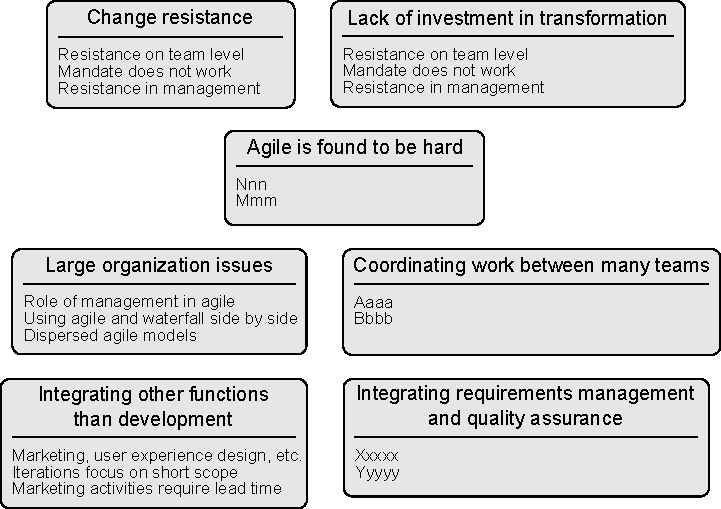
\includegraphics{graphics/challenges_summary.pdf}
    \caption{Overview of challenges in agile transformations}
    \label{fig:challenges_summary}
  \end{center}
\end{figure}

The challenges found in the primary studies are summarized in figure
\ref{fig:challenges_summary}. The challenges are organized on a high level into
seven categories within three themes. The categories are discussed subsequently
in this section. First we present generic transformation issues that may apply
to any organization. As the second theme challenges relating particularly to
sizable organizations are discussed. The final theme studied is challenges
encountered when agile development needs to interface with other functions
involved in a system development life cycle.

It is to be noted that we do not emphasize any of the listed categories or
challenges above another. The challenge categories we present were found evenly
in the set of primary studies. We included only challenges that had been
mentioned in several studies, or were particularly emphasized in fewer studies.
Challenges with only sporadic mentionings were considered less significant and
were left out. There was no further evidence that any challenge would be more
significant than another.


\subsection{Change resistance}

In an organizational transformation working habits and roles need to change.
However, people are usually disinclined to change and some resistance should be
anticipated in any change process. People will not be willing to change unless
there are good reasons, and the change is perceived easy enough. It is difficult
to attain a buy-in for a change, and even organizations that have a flexible
culture will face resistance [P10]. It should be expected that not everyone will
be willing to change, even so that some employees will never adapt to the new
model [P6]. During a transformation period objections to change may become a
major reason for loss in time and productivity [P29]. The main types of change
resistance discovered in the primary studies are summarized in table
\ref{table:challenges_changeresistance}.

\begin{table}[b]
    \centering
    \begin{tabular}{ l l }
        \toprule
        Types of change resistance           &  Described in  \\
        \midrule
        General resistance to change         &  P14, P18, P22, P44, P45   \\
        Skepticism towards a new model       &  P5, P8, P9, P18, P36, P46 \\
        Top down mandate creates resistance  &  P2, P12, P37, P49 \\
        Management not willing to change     &  P2, P3, P6, P49 \\
        \bottomrule
    \end{tabular}
    \caption{Types of change resistance reported in studies}
    \label{table:challenges_changeresistance}
\end{table}

Numerous reasons were given for why change resistance emerged. For
instance, Fecarotta [P14] described the organization of Boeing as risk-averse
and cautious, which slows down any change. Any change was further hindered by a
deeply rooted status quo and high employee retention [P14]. In some cases it was
reported that people worried about new roles and responsibilities that the agile
model might bring [P44]. For instance, testers were worried that they would need
to take on cross functional tasks, which would be outside their area of
expertise [P18]. Yet another reason for change resistance was the move from own
offices to team areas [P22]. People were also feeling being monitored because of
the increased level of interaction within the team and between project
stakeholders [P45].

In these cases change resistance was mitigated for instance by education [P45]
and one-to-one discussions [P22]. Change resistance was also softened by first
engaging only teams willing to try agile, so that insights could be gathered to
ease the continued transformation [P45].

Another common form of change resistance that was reported was skepticism and
distrust in suitability of agile. Seffernick describes how management did on one hand
acknowledge benefits of agile, but on the other explained away the possibility
to apply it due to contract reasons, the current matrix organization, and other
organizational practices [P46]. Skepticism was often created by other similar
misconceptions, including that agile does not work for complex products [P5,
P36], agile needs to be implemented in a prescriptive by-the-book way [P9], that
frequent meetings will cause overhead [P18], and that agile equals avoiding
governance and working without a plan [P8].

% For instance, teams may not be willing to try
% new approaches unless they have been proven [P6]. 

% Resistance is to be expected --> there are many different stakeholders [P41]

% * No value seen by some groups, e.g. mainframe or maintenance [P49]

The way the transformation is initiated will affect how change resistance will
show. In several cases the change initiative came from management, but when
presented wrong the initiative becomes a mandate that people are not receptive
for. Spayd [P49] summarizes this as: ``Organizations do not change merely
because the boss says so, at least not in the way that is intended''. In that
organization the introduction of CMM had been carried out consistently by a
mandate, but the collaborative nature of agile did not mix well with such a
mindset. A top down mandate may also dilute the understanding of the reasons for
starting the transformation, and the understanding of agile development overall
[P2]. O'Connor describes how team members became skeptical towards agile when
implementing mandated changes did not bring any visible benefits [P37].
A problem relating to top down mandate is that if management does not speak out
a goal towards using agile, developers may feel that the agile methods may be
replaced by something else at any time [P12].

The direction in which a tension between management and development is built may
also be opposite. In cases where the change was emerging bottom up the
reluctance to change was not in the team members but management, causing that
significant organizational change could not be raised above the team level. For
instance, Atlas [P3] describes how executive support would have been required to
extend the agile process to involve the product management office and separate
quality assurance groups. In this case, when managers %for multi team projects
were not involved in the transformation, the agile model was restrained from
spreading beyond the level of development teams [P3]. Lack of middle management
support for change and disinclination to change management culture were seen as
some of the most serious problems in the transformation [P2, P49]. Middle
management is in a position to undermine the entire transformation, and may do
so if they do not participate in, and thus understand, the agile method. Agile
brings changes to some management roles [P2], and lack of understanding of agile
development will leave managers feeling left out [P6].


\subsection{Lack of investment in transformation}

It is clear that changing the way of working will create some costs for the
organization. Problems will ensue if there is no intention to allow resources
for the transformation. Table \ref{table:challenges_lackofinvestment} presents
investments and resourcing arrangements that were withheld, and which caused
problems in transformation.

\begin{table}[b]
    \centering
    \begin{tabular}{ l l }
        \toprule
        Factors of investment and resourcing  &  Described in \\
        \midrule
        Lack of coaching                      &  P1, P6, P23, P45, P47, P49  \\
        Lack of training                      &  P11, P20, P45  \\
        Excessive commitment of people        &  P37, P42, P49  \\
        Old commitments are kept              &  P11, P21  \\
        Physical spaces can not be rearranged  &  P6, P14, P29, P36, P38, P49  \\
        \bottomrule
    \end{tabular}
    \caption{Summary of investment and resourcing factors that affect
             transformation negatively}
    \label{table:challenges_lackofinvestment}
\end{table}

% Lack of training and coaching 

Training and coaching are direct investments in transformation and their lack is
an evident problem. These activities were still under budgeted, which
created difficulties in the transformation [P11].
Hajjdiab [P20] describes how reluctance of management to invest in training
caused teams to be ill prepared for the agile transformation effort, which
eventually resulted in ending the use of agile methods. As a less dramatic
outcome of too little training was lower motivation [P45].

Arranging proper coaching was a particular problem in many organizations. It is
critical to coach teams in their real work environment as a proper change in
mindset is difficult to achieve by only attending training sessions. [P9, P23]
In large
organizations where numerous teams needed to be coached the demand often
exceeded the capacity of available coaches [P1, P6, P23, P49]. Lack of coaching
was also attributed as a reason why the success of pilot teams could not be
repeated when agile was adopted more widely [P9, P45].
Silva and Doss [P47] described that when it was hard to fill the coaching
positions people less seasoned in agile were appointed as coaches, which risked
that agile practices would not be taught correctly.

% Add quote?
% * No coaching --> Applying techniques improperly --> Damage
% [P9]
% Without proper coaching however, the success of these informal teams met with
% mixed results over the longer term.  In retrospect, many of these teams did
% damage to themselves by improperly applying Agile techniques, particularly when
% command and control mechanisms were still in place.


% Old work and commitments, schedule pressure

Even though the organization was in a state of transformation the workload of
teams was not always adjusted to facilitate the process.
Some organizations started their agile journey in a state where people were
over-committed. It was later realized that when people are overloaded they will
not be able to changing their behavior and learn new ways of working [P37, P42].
Spayd [P49] also describes how senior management pressed teams to deliver what
the customer had been promised, regardless of what the current velocity of
development predicted. For one part the pressure to deliver interfered with the
transformation, but it was also forcing a change in the old way of working
[P49].

In one case management forced people to remain committed to firm deadlines, even
midst in the organizational transformation [P21]. The engagement in old
commitments and tasks resulted in ignoring new practices introduced by agile,
and eventually the agile method was breaking down [P21].
Cowan [P11] describes how time was allocated for tending to old commitments.
However, even when there was preparation for extra work people with specific
expertise became overloaded. After time it was realized that over-commitment must
be reduced by allowing to shift excess work for later time [P11].


% Physical spaces, challenge of finding a seating

In some cases the old way of working had people seated physically distributed,
in opposite to what agile methods typically suggest. Office spaces needed to be
arranged so that the entire team could work in a single room, but it took time
and effort, and it was not always possible [P6, P14, P36, P38]. Lewis and Neher
describe how dedicated rooms for teams could not be arranged, and team events
such as daily stand-ups required booking a conference room [P29]. In another
case the estate organization shut down the teams' attempts to modify working
spaces [P49].


\subsection{Agile is difficult to implement}

A challenge most organizations came across was that implementing the agile model
was found to be difficult. An experienced software team may do well in training,
but when the time comes to apply agile techniques in practice the team may get
lost [P21]. Viewpoints on the difficulty of correctly implementing an agile
model are summarized in table \ref{table:challenges_difficulty}.

% The difficulty in implementing agile is evident in misconceptions of the agile
% model, when by-the-book implementations prove to be insufficient, and when the
% agile methods were applied badly to the organization.

\begin{table}
    \centering
    \begin{tabular}{ >{\raggedright\arraybackslash}p{0.51\textwidth}
                     >{\raggedright\arraybackslash}p{0.41\textwidth} }
        \toprule
        Type of difficulty in implementation  &  Described in \\
        \midrule
        Misunderstanding agile development concepts  &
                P6, P26, P37, P38, P42, P44, P45, P48, P49      \\
        Literature does not provide enough guidance  &
                P5, P6, P10, P13, P21, P27, P30, P45, P49     \\
        Agile practices are customized badly   &
                P9, P29, P44, P46  \\
        \bottomrule
    \end{tabular}
    \caption{Summary of viewpoints why agile implementation is difficult}
    \label{table:challenges_difficulty}
\end{table}


% Misconceptions of agile

There were many examples on problems caused by misconceptions of what agile
software development is. On a general level, Bang [P4] describes how the values
of the agile manifesto were not understood, and agile practices were carried out
without understanding their purpose. In one case management saw the purpose of
agile simply being faster product delivery [P9].

On a team level there were several examples of misunderstanding agile
development. Cases describe how agile was seen as freedom to hack without
documentation [P26], that development could be done without design tasks [P37],
and that agile meant that everyone should become a generalist [P42]. Schatz and
Abdelshafi describe how teams presented unfinished work at reviews and ignored
the principle of showing only completed increments, which resulted in a backlog
of bugs [P44]. In one case team members had perceived the introduction of agile
as a means to squeeze out more efficiency [P45]. In addition, the flatter
organization was seen as fewer career opportunities, and pushed team members to
internal competition for visibility [P45].
Still one misunderstanding of agile was due to viewing it only through the tools
used, such as project management software [P48]. Superficial focusing only on
tools themselves and not the reasons behind their use led to frustration [P42].

In some cases the misunderstanding of the agile model was described as ``doing
mini waterfalls'' [P6]. Managers were using Scrum terminology, but at the same
time committing unreasonable workloads on teams [P6]. In another case a
waterfall nature was evident when task estimates were given as hours left, and
task breakdowns disconnected from what was really being done [P27].

As a final example of misconceptions, some organizations considered agile being
a solution to all problems [P9]. Success was declared prematurely [P49] but
expectations created by successful early experiments were not fulfilled [P38].
Disappointment was granted when these hopes were not fulfilled, and instead
implementing the agile model was found to be hard and time consuming.

% By the book is not good

Even if there was no misunderstandings the correct agile model was hard to
implement. Several cases describe how an agile model was hard to learn from
literature [P21, P27], especially when it comes to implementing it on a large
scale [P13]. As Beavers [P5] writes: ``There simply was not a manual or document
where we could find easy answers on how to do things''.
Schnitter and Mackert [P45] report that theoretical considerations on how to
scale up the agile methods were not good enough, and that product managers and
architects struggled when several Scrum teams were working concurrently.
Another case concluded that all practices suggested by XP did not fit enterprise
scale development, and some practices required customization [P49].

% In a large organization with several different teams and projects it is clear
% that one single model can not fit all needs [P41]. The model of
% agile should not be prescribed in a strict way, as it would impose a single
% model in an organization with several individual teams and projects [P41].

% Check this paragraph
Further indications were given that the advice from literature will not ferry
all the way. Benefield [P6] describes how it was difficult finding a balance
between prescribing a by-the-book implementation which may put people off, and
giving too much freedom in the agile methods which may weaken core practices.
The reality where the practices needed to be applied was described as messy in
comparison to the ideal circumstances presented in literature [P10]. Because of
this it was difficult to choose a model to start with and gain buy-in for [P10].
Difficulties in choosing a initial model were also due to variances perceived in
the agile approaches suggested in literature [P30].

% Where would this belong?
% Organizations had also bad experiences if the implementation of the agile model
% was being prescribed. For instance, implementing Scrum based on checklists of
% practices would not work [P41]. Benefield described that it was challenging to
% find a balance between independence for teams to choose their way and diluting
% the value and structure of Scrum [P6]. Giving room for team autonomy is one of
% the critical facets of agile, but it must be ensured that teams do not discard
% practices that add value and structure.

% Customizing badly (mapping to old model)

The difficulty of agile and misunderstandings were also evident in cases where
the methods were customized badly. As by-the-book implementation often was not
feasible, the agile method was tailored to suit the needs of the organization.
However, in some cases tailoring meant skipping some practices, which lead into
problems. In one case certain individuals were allowed to ignore some core
elements of Scrum, which came to turn the teams decision making into a variant
of command and control [P9].
Lewis and Neher [P29] describe how there was temptation to strip some practices
and enhance others. Previous attempts had proven that one of the reasons for
agile implementations to fail was deviations from the process, because of which
the agile mindset did not take root [P29]. A bad customization may lead to the
team taking only practices that reflect their current needs, and therefore
failing to achieve a real change in process and mindset [P9, P46].
Another example of bad customization that counteracts change is replacing agile
vocabulary in favor of familiar terminology from the old model [P44]. An
important benefit of introducing new vocabulary is that it stimulates new ways
of thinking [P44].


\subsection{Coordinating work between many teams}

In large software projects work must inevitably be distributed between many
teams. One of the most prominent transformation challenges was the difficulty in
creating a model to coordinate work between many teams. Table
\ref{table:challenges_coordinatingteams} presents challenges that arose when
agile was implemented in environments where many teams need to collaborate.

\begin{table}[h]
    \centering
    \begin{tabular}{ >{\raggedright\arraybackslash}p{0.61\textwidth}
                     >{\raggedright\arraybackslash}p{0.31\textwidth} }
        \toprule
        Problems in environments with many teams  &  Described in \\
        \midrule
        Interfacing between teams is difficult     &  P9, P10, P13, P17, P24, P26 \\
        A model with autonomous teams is not good  &  P7, P13, P29, P51  \\
        Distributed setting causes additional problems  &  P29, P45, P48  \\
        Technical integration and consistency      &  P5, P24, P26, P27, P50  \\
        \bottomrule
    \end{tabular}
    \caption{Summary of challenges in a setting with many agile teams}
    \label{table:challenges_coordinatingteams}
\end{table}

Many cases reported that introducing agile practices soon yielded improvements
on the team level, but as a part of a large transformation teams also needed to
change their external behavior.
The initial success was followed by challenges when teams needed to work with
other teams and as parts of the larger surrounding organization [P13, P17, P24].
Introducing agile had created flexibility on a team level, but it could not be
fully utilized as the surrounding organization was not responsive enough [P26].
The roll-out of agile had not removed dependencies, and the dependencies
made managing development difficult [P9, P10].

% Independence of teams

Some organizations attempted to initially create a model where teams operate
autonomously, which is well in line with agile principles. However, a number of
issues arose from independence. For instance, teams needed to find a balance
between the their own goals and broader goals of the entire organization, but
some teams chose to focus only on their own goal [P7]. Coordination was
obstructed by independent teams that did not respect the larger context [P13].
Coordination was also difficult when teams were working independently for
different customers but the applications being built were interdependent [P29].
One case reported that even allowing teams to have different sprint durations
created delays in delivery [P51].

Further coordination problems were encountered when scaling up agile over many
sites. Operating in a distributed environment makes communication more
difficult, and causes problems when frequent and effective communication needs
to be achieved. Distribution had negative effects, such as missing kick-off
meetings, reduced feeling of proximity when telecommunication is necessary, and
difficulty in arranging frequent meetings due to time zone differences [P45].
Agile project management was also problematic in a distributed setting. In a
waterfall model separate parts of projects could be isolated to different sites,
but the agile model does not allow such strict slicing of projects [P29]. In one
case it was simply admitted that a distributed organization will impose
additional burden on communication and require additional care in the process,
but distribution and agile would still be used together [P48].

Also technical problems relating to inter-team coordination were reported.
Integrating the products of teams was seen as a problem in some cases [P5, P50],
and lack of standardized build scripts was mentioned as a problem in one case
[P27]. There was also problems in synchronizing definitions of software
interfaces between teams, and dependencies in code caused problems in larger
features [P26]. One case reported that team centricity in the agile model
created a fragile architecture, divergence in coding style, and even distrust
between teams [P24].

Moore and Spens [P34] describe the progression of the above mentioned
coordination problems. At first cross-team dependencies were attempted to be
reduced, but it became evident that the dependencies were an inherent part of
the project. A traditional approach to managing dependencies created excess
work, reduced independence and flexibility of teams, and created contract based
and adversarial relationships within the organization. There was some success
when up to 5 teams were coordinated using Scrum-of-Scrums, but that model could
not be scaled to a global level. The main problem was teams that were thinking
too much inside the team walls. When the new practices were scaled up the
communication channels narrowed and created communication breakdowns. Problems
with collaboration, dependencies, and integration were solved in the presence of
individuals having a proactive and open mindset towards working over team
boundaries. It was concluded that a balance is needed between completing new
stories from the team backlog and maintaining overall stability of the
application. [P34]

Many studies presented solutions for the inter-team challenges, which also
highlight the nature of the challenges themselves. The general model of solving
inter-team problems was introducing an additional layer of coordination, such as
a Scrum-of-Scrums team [P43], a similar product team [P45], or an entire
customized release framework [P13]. In one case integration problems were
controlled by prioritizing code quality and maintaining existing functionality
over new features [P13]. Finally, the choice of tools was reported to have an
impact on the coordination effort [P17].



\subsection{Issues specific to large organizations}

In addition to inter-team coordination there were also other challenges that
should only emerge in a sizable organization.
Most importantly, additional layers of management are usually necessary to steer
large groups of people. The problem is that agile methods provide little
guidance on how to organize management.
Problems may also arise in a large environment if the schedule of agile adoption
varies from team to team. Internal fragmentation is a further problem that may
be encountered in large organizations.
Table \ref{table:challenges_largescale} summarizes these challenges.

\begin{table}[t]
    \centering
    \begin{tabular}{ >{\raggedright\arraybackslash}p{0.56\textwidth}
                     >{\raggedright\arraybackslash}p{0.36\textwidth} }
        \toprule
        Challenges relating to large scale  &  Described in \\
        \midrule
        Management roles unclear in agile       &  P2, P11, P27, P30, P38, P49, P52 \\
        Using old and new models side by side   &  P1, P8, P10, P26, P29 \\
        Management uses waterfall model         &  P3, P6, P35, P38, P45, P46 \\
        Duplicating management with two models  &  P20, P48 \\
        Agile models diverge between teams      &  P8, P9, P38, P43, P48 \\
        Internal boundaries in organization     &  P10, P11 \\
        \bottomrule
    \end{tabular}
    \caption{Summary of challenges relating especially to large scale}
    \label{table:challenges_largescale}
\end{table}

% Roles of managers

The existence of additional management positions may pose problems to agile
processes that emphasize self organization.
Especially the role of middle management was unclear in agile methods [P2]. This
is problematic as an agile transformation requires cultural change particularly
on the middle management level [P2].
It was described that managers needed to resist the tendency to take command and
control and allow room for self organization, but the change in role was
difficult to achieve for the people involved [P11, P52].
Nielsen and McMunn [P30] describe how the project management group had
previously worked through big up front plans and competing of resources, but
those ways would need to dramatically change.

Several other problems related to management roles were also presented. For
instance, Spayd [P49] describes how managers were left outside the roles offered
by the new agile model. In another case when managers were appointed as Scrum
masters developers felt being micromanaged [P27]. This was partially because of
vague understanding of the agile method [P27]. It was also described how mixing
the role of project manager and Scrum master created a conflict in interest, and
turned the Scrum manager's role into one of policing the team instead of
supporting the team [P30]. In some cases problems with manager positions were
solved by phasing out roles relating to the old model, and replacing them with
new positions more suitable for agile [P38, P52].

% Using two models side by side
% Part of the organization is in old mindset

In most cases a large organizational transformation proceeded gradually, and
during the process it was possible that the new agile model was used in parallel
with the old methods. The arrangement of using the old and new models side by
side was seen as generally problematic [P1, P26], and causing tensions on all
organizational levels [P10]. Ongoing projects had been set up with previous
development methods, and the agile methods needed to be arranged to fit along
with them [P8, P29]. A particular problem in collaborating between projects
using different models was that in Scrum the software design was fleshed out
over time as sprints progressed, but the waterfall model would require detailed
design to be locked early in the project [P29].

Even when agile had been taken into use in development there were problems with
management working according to the old waterfall model. O'Connor [P38]
described management as ``focused on meetings and big up front project plans''
despite agile being in use. In another case management was losing confidence in
agile because familiar reports on cost analysis and percentage complete were not
produced [P35]. As Scrum teams did not commit to fixed schedules they were
considered unreliable according to the original model [P45].

Some cases reported that development efforts were still controlled on a top
level by a project management office (PMO). The PMO was described as entrenched
in a waterfall paradigm, and the top-level rigidity was causing friction in the
agile adoption [P3, P6]. The PMO was seen as a hub and bottleneck controlling
all aspects of projects, and its central structure had to be dismantled for the
organization to become agile [P46].

There were also problems with duplicating management when two models were in
effect. For instance, agile teams were required to comply with current
procedures producing excess documentation and stepping through approval gates
[P20, P21]. The bureaucracy of the previous traditional model was still enforced,
and management was not convinced to lighten the process. Another case describes
that after introducing the agile method teams were required to fill in templates
of two processes [P48].

% Challenge: Differing vocabularies

In addition to teams using agile and waterfall models side by side a large
organization makes it possible that the agile interpretations of teams diverge.
When many teams implement agile without consistent guidance friction and
fragmentation may emerge [P9]. The organization may require moving people
between teams from time to time, and therefore it would be desirable that no big
differences in teams' agile cultures exist. Divergence in process would create
risk of increased costs when relocating people [P38].
Further, if processes of teams diverged management had difficulties in
forecasting and comparing work of different teams [P38, P48]. To overcome
problems with divergence in agile models some organizations defined standards to
follow [P8, P43].

% Challenge: Previous organization in silos is haunting new model
% Is this good??
In some cases the initial organization had internal boundaries or specialized
knowledge was stuck silos. Such settings caused problems in the agile
implementation.
Cloke [P10] describes how use of Scrum revealed an internal segmentation where
teams operated with differing priorities and agendas. This segmentation also
hampered the initial effort to use Scrum in a larger context [P10].
Cowan [P11] describes how projects needed specialized skills that were scarce
and people were often relocated to match the needs of the moment. Too much
reorganization made it difficult for teams to plan ahead [P11].

%% This??
% A dispersed matrix organization causes problems when people are on one hand
% kept assigned to many projects simultaneously, but on the other hand functions
% such as database administration, architecture boards, and project management are
% centralized [P14].

%% ?? -->
% Large organization put agile methods under the test of scaling up, and problems
% were encountered.
% In the agile model it was hard for managers to get an overview of the progress
% of the release [P17]. The status of features was hard to tell because different
% aspects of features were sepatated across teams [P17].
%
% One case reported use of agile across hundreds of teams, but management could
% not get a roll up of the progress without having strict rules on how status was
% reported [P48]. Schnitter and Mackert [P45] report that a maximum workable size
% in a project managed by Scrum was 130 people including 7 development teams.
% Smits and Rilliet [P48] report that providing executive overview of the
% development programs was limited by the tools used to manage agile projects.

% --

% Add quote ?
% * Especially higher organizational levels were not using agile --> Problem
% [P3]
% Scrum still exists mostly in a way that avoids conflict with the larger
% corporate organization, and there has been little progress in addressing larger,
% organizational impediments.

% [P18]
% Real Agile teams will experience resistance when they start working with
% non-Agile interfaces. Lack of understanding in ‘why to help create a cadence?’,
% ‘why involve the customer more?’ will cause resistance in the change process.

% --> ``Part is in the old mindset''
% * Problem: Management attempts to use a ``resource pool'' of individuals rather than coordinating teams
% [P6]
% we face the constant threat that restructuring and the instinct from management
% to track and leverage resources at the individual level (for example
% organization-wide resource pools) will destroy the team dynamic and adversely
% affect productivity.


\subsection{Integrating requirements management and quality assurance}

% TODO:
% * Mieti rakenne
% * Mieti onko seuraava ``other than development'' hyvä otsikko


Development is traditionally preceded by requirements engineering and succeeded
by quality assurance (QA) activities. Agile methods suggest that essential parts
of these activities would be performed within the development team. However, for
large systems the effort required for managing requirements and QA may be too
heavy for individual teams to handle. For instance, a single development team
can manage and elaborate items in its own backlog, but a large feature may
require work across many teams. The feature needs to be divided to team specific
items on a higher level, and the process must be managed somehow.
Table \ref{table:challenges_requirementsandqa} presents challenges in
implementing additional requirements management and quality assurance required
in large development projects.

\begin{table}[!b]
    \centering
    \begin{tabular}{ >{\raggedright\arraybackslash}p{0.61\textwidth}
                     >{\raggedright\arraybackslash}p{0.31\textwidth} }
        \toprule
        Challenges in requirements engineering and quality assurance  &  Described in \\
        \midrule
        How to accommodate high level requirements management  &  P24, P31, P39, P45, P51  \\
        Problems with breakdown of requirements        &  P1, P17, P33, P48  \\
        Creating and estimating user stories is hard   &  P5, P11, P27, P30, P33, P37 \\
        Handling coexisting long and short term planning  &  P9, P10, P13, P26, P31, P38 \\
        Accommodating performance, load, and memory testing  &  P17, P28, P31, P48 \\
        Lack of automated testing slows down           &  P10, P11, P17 \\
        New requirements management practices affect QA  &  P5, P48 \\
        \bottomrule
    \end{tabular}
    \caption{Summary of requirements engineering and quality assurance related
             challenges relating in the agile model}
    \label{table:challenges_requirementsandqa}
\end{table}

% Requirements engineering is difficult

In agile methods requirements engineering is usually informal and closely tied
to the development team. However, large development projects will demand
additional high level requirements management. This is apparent in cases where
complexity of the product will require additional layers of product management
[P45], requirements are created by several stakeholder groups and development
teams can not be in contact with all of them [P39], or teams do not have access
to stakeholders due to a distributed setting [P24]. Agile methods need to be
extended to include a process on how to get large requirements into team
backlogs [P31].

Requirements were in some cases first defined on a high level in marketing
requirements documents (MRD) [P1, P31] or functional specifications [P33].
These high level requirements needed to be elaborated to be used by agile
development teams. The requirements breakdown in it self was found to be
difficult [P1, P33], and also when to do the breakdown and to which detail level
[P17].
Product managers and business analysts were struggling in creating high level
requirements [P33, P37, P51], and teams were struggling in breaking them down to an
estimable size [P33]. Smits and Rilliet [P48] describe how high level product
management delivered requirements in too large chunks resulting in development
teams spending large amounts of time on defining suitably sized stories.

Several cases highlighted that much learning was needed to master the new
process of creating user stories, both on product management and development
levels [P27, P30, P33, P37]. There were problems such as ambiguity in
requirements [P5, P11], and effort estimation for stories was hard to do well
[P27, P37].

% As an integral part of the software development lifecycle, requirements
% management will be affected by the new agile process. In large organizations
% product and requirements management was initially done in a traditional way, but
% it was contrasted by the agile process that required iteratively supplying small
% requirements to development [P51]. 

% In one case the teams were overwhelmed by reprioritization and requirements
% bartering when stakeholders learned that requirements could be rearranged
% flexibly [P31].

% Long term planning

High level requirements work and estimation was problematic as there was a gap
between short and long term planning [P9, P10]. Typical agile backlogs would
give only short term visibility, so organization specific practices for long
term planning had to be created [P26, P31]. Several cases described that care
had to be taken to avoid long term planning becoming a prescriptive practice. In
order to preserve the agility of development a schedule driven approach was
avoided [P10], sensitivity was used when considering setting milestones [P13],
and striving for more accurate estimates was not let to become an excuse for
gathering requirements up front [P38].

% Problems with enterprise or external QA

In an enterprise setting quality assurance tasks will require effort beyond the
general agile convention of doing testing within a cross-functional team.
Similarly as with requirements engineering, the agile model may need to be
extended to accommodate additional testing activities [P31]. Organizations may
have existing separate QA teams that must be coordinated to work with
development teams [P17, P30, P48]. Integrating enterprise scale QA will pose
some additional challenges to agile methods.

Full quality assurance of a system requires special testing such as performance,
load, and memory testing, but agile methods lacks focus on them [P17]. These
testing activities can not be done within boundaries of user stories, and
require more resources than teams can spare [P31]. When testing tasks overlap
team boundaries it is sensible having a separate teams for the tasks, but
coordination practice between specialized QA teams and development teams needs
to be defined [P28, P48].

Some cases reported on problems with lack of automated testing. For a large
system the lack of automated tests caused excess testing work and late discovery
of defects [P10, P11, P17].

Still one challenge in QA was the relationship to requirements engineering. The
QA functions were struggling if there was problems such as ambiguity or
ineffective breakdown of large requirements [P48]. In a waterfall model an
extended time was reserved for QA at the end of projects, which allowed to
retroactively resolve ambiguities in requirements [P5]. However, ambiguity
became an impediment to QA when development worked in short increments and
there was no extended period for stabilization [P5].


\subsection{Integrating other functions than development to agile}

Agile methods are typically considered as a set of activities closely related to
software development. Cases describe how development teams were the first
entities that were considered when introducing agile [P2, P17, P31, P38].
However, development operates in a larger context and will need to interface
with other organizational functions.
Challenges were faced when exposing other parts of the organization to the agile
model, and functions that were further away from development were resistant to
change [P2, P18, P31]. A tension was growing between development and broader
roles in the organization [P1]. The full benefits of the transformation would
not be attained unless the entire organization was set to work along the same
paradigm [P18, P42].

Primary sources listed various functions beyond development that are involved in
bringing products to the market. Functions interfacing with development and
affected by the agile transformation are presented in figure
\ref{fig:challenges_other_functions}.
Marketing was a particularly frequently mentioned group [P5, P17, P28, P31, P38,
P45, P48]. Other groups involved in the whole of product delivery were sales
[P17, P31], infrastructure and operations [P10, P45, P46, P50], user experience
and design [P9, P10, P28], documentation [P28], legal [P10], security [P10],
customer services [P48], and finance [P48].

\begin{figure}
  \begin{center}
    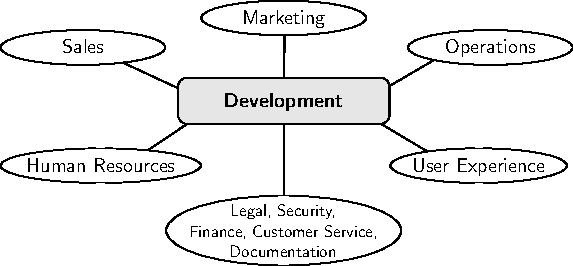
\includegraphics{graphics/challenges_other_functions.pdf}
    \caption{Functions affected by the agile transformation}
    \label{fig:challenges_other_functions}
  \end{center}
\end{figure}

Agile affects timings in the software delivery life cycle, what caused two types
of problems. Firstly, the iterativeness of agile models was problematic when
interfacing with other functions. Iterativeness changed the pace of delivery
[P17], and forced design to focus on a shorter scope [P15]. Various groups
feeding and supporting development had earlier committed once to a long term
plan, but in the new arrangement they needed to adjust to incremental delivery
[P48].
Especially user experience (UX) and interaction designers did not welcome an
incremental model [P6], and were struggling with maintaining the big picture in
design while working in iterations [P9, P10].
The infrastructure and operations teams were falling behind due to the increased
delivery speed of development teams, and they were forced to update their way of
working [P46, P50].

Federoff and Courage [P15] elaborate on the user experience team's problems
with the short time horizons of Scrum. Previously the UX team had supplied
development with designs within a long release cycle, but Scrum required
completing features within weeks. The problem was that that the UX work required
a holistic view instead of an incremental one, and the design process did not
fit well into the time frame of a sprint. The UX team was overloaded and
discontent, but the situation was fixed by refining the schedule for interactions
with development teams. [P15, P28]

The second type of problems was that some release activities would inevitably
have a long lead time but required committing to a set of functionalities in
good time. The agile model's emphasis on short time horizon and flexibility in
prioritization did not mix well with such activities.
For instance, it would take time to prepare printed marketing material and press
releases, but they needed to accurately present the upcoming features of the
product [P38].

Maples [P31] describes that marketing needed three months for preparing the
product launch, but the agile process allowed development to keep changing the
content of the product. As a result marketing was struggling with creating
material and campaigns without knowing the exact product features. Further, the
processes of acquiring export clearances and licensing authority required that
the the feature set of the product was known well on beforehand.
As a result of these requests development felt that their process was being
slowed down. The issues were solved by agreeing on that marketing could at any
time request a release in 90 days, and development would be able to commit to a
fixed feature set to be delivered [P31].

% Problems with HR

Problems in adopting agile were even showing in functions outside the software
delivery life cycle. In several cases human resources (HR) was a support function
mentioned to work against the agile adoption. In order to gain full results of
the transformation the entire organization should to be aligned, including HR
[P38, P42, P49].
Especially the rewarding practices set by HR were seen as problematic for the
agile model. Rewarding was tied to personal performance, which was acting
against team centric thinking and the agile model in general [P3, P6, P49].
One case reported even on a practice of tracking failures down to individuals
[P40].


\subsection{Other challenges in transformation}

There were still some other challenges in the transformation that do not fit in
the categories presented above. Two particular problems are worth mentioning.
Firstly, there were certain factors that pulled people back to the old ways of
working, and secondly, excessive enthusiasm in agile had negative effects.

% Falling back to old model

In several cases challenges in the transformation resulted in people falling
back to the old model of working. In some cases it was only a temporary struggle
while learning agile practices, but in other cases the old model displaced
agile.
Development work has to go on during the transformation but there will be new
things to learn for the team. Stress caused by the combination of schedule
pressure and much change at once will pull people back to the old way of working
[P11, P18, P38].
Schatz and Abdelshafi tell how even subtle trouble may risk the transformation,
as people will always look for reasons to revert to familiar behavior [P44].
Teams without adequate training were struggling with applying agile practices
correctly, and the challenge the new practices posed made people to abandon them
and return to the ways they know [P6, P49].

In some cases agile was seen as an overhead, and was therefore abandoned. For
instance, as new practices were being introduced there was a decrease
performance, and when teams realized that the benefits are not immediate they
started reverting to the old model [P21].
Evans [P12] describes that new senior appointments changed the management to be
less favorable towards agile, and a waterfall development model started to
return.

% Agile zealots

A phenomena that troubled some organizations was over-enthusiasm towards agile
methods. In several cases there was mentionings about change leaders or teams
becoming agile zealots. For instance, Evans [P12] describes how some members of
the agile community were becoming too evangelic, which made people take sides
for or against agile development. In another case team members started out with
an overly eager attitude, but when agile did not deliver improvements the
interest faded and started to go back to the old process [P20]. Attempting to
implement agile too strictly may cause conflicts, and especially in a large
organization the change leaders need to maintain a collaborative attitude
towards various groups in the surrounding organization [P6]. Introducing agile
methods does not guarantee success, and therefore they should not be followed
blindly [P4].


% When a release schedule with fixed deadlines that business required was combined
% to agile managers started to behave authoritatively and the self organization of
% agile started to break down [P31]. % (Skeptics used this as a sign of that agile can not work)

% This??
% % People do not speak their minds
% In one case a passive-aggressive organization culture was described as a
% challenge. Ranganath describes how people did not speak their minds in meetings,
% thus creating a false sense of agreement when talking about how the organization
% should develop. Because of this resistance and concerns were left growing, and
% acted against achieving a successful transformation. To to avoid these issues
% change leaders worked with team members on an individual level to win confidence 
% and make their voices heard [P40].



\clearpage

\section{Success factors in transformation}

The analyzed primary studies brought up several factors that contributed in
success in the transformation. As stated by Research Question 4, we studied what
factors were reported to facilitate the transformation process. We present
factors that the primary studies particularly highlighted as being important in
advancing the transformation process.

\begin{figure}[!b]
  \begin{center}
    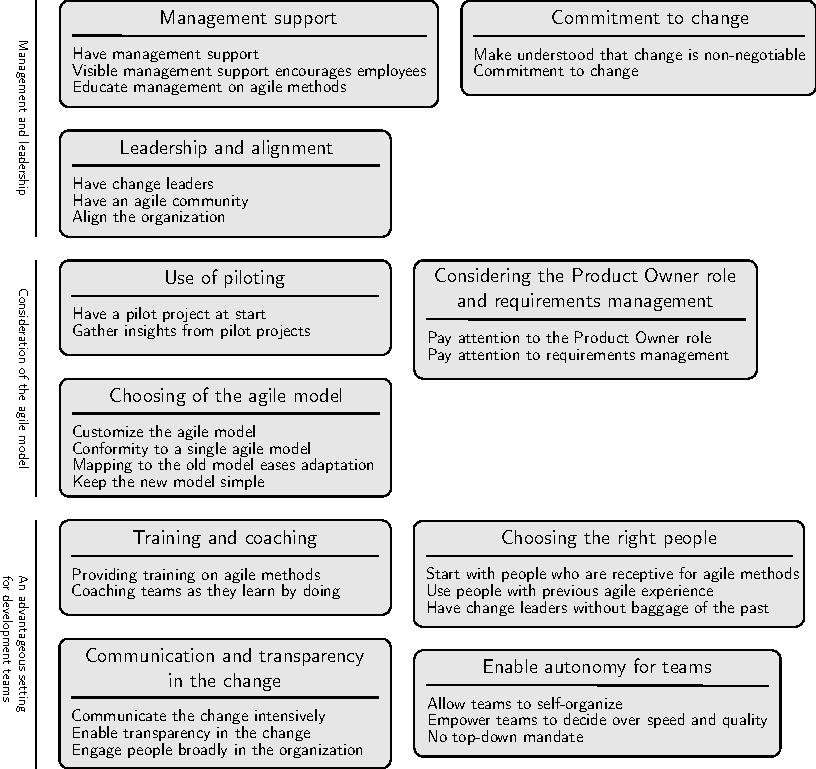
\includegraphics[width=1\textwidth]{graphics/success_summary.pdf}
    \caption{Overview of success factors in agile transformations}
    \label{fig:success_summary}
  \end{center}
\end{figure}

Figure \ref{fig:success_summary} summarizes success factors evident in the
primary studies. The success factors are organized into ten categories within
three themes, which are elaborated in this section. The first theme relates to
management and leadership in the transformation. The second theme presents
success factors that relate to finding a suitable agile model for the
organization. The last theme includes success factors that are realized on the
level of development teams.

The discovered success factors did not exhibit strong differences in
significance in respect to each other. Three categories of success factors can
be considered of higher importance: management support, training and coaching,
and choosing the agile model carefully. The remaining success factors should be
considered having even significance.

% * What is our standpoint on recommendations that experience reports give, but
%   which were not necessarily tried in the organization?
% 
% * Some success factors are just calculated decisions that were made because
%   the organization saw them as the best way to proceed. The question whether
%   the decision really were critical for success is not proven. 
% 
% * Some success factors are compiled from ``what we learned'' or ``advice for
%   others'' lists. We considered whether the advice was something the
%   organization had tried in practice.
% 
% * For instance, implementing continuous integration and automated builds was not
%   explicitly stated as a factor contributing to the success of the
%   transformation, although it is unquestionable that such systems are critical
%   for maintaining quality and enabling frequent releases.


\subsection{Management support}

The most prominent and clear success factor was having support from management.
When the leadership of the organization is committed and supportive change is
much more likely to happen. Table \ref{table:success_management} lists
success factors related to management support.

\begin{table}[h]
    \centering
    \begin{tabular}{ >{\raggedright\arraybackslash}p{0.41\textwidth}
                     >{\raggedright\arraybackslash}p{0.51\textwidth} }
        \toprule
        Success factors  &  Described in \\
        \midrule
        Have management support  &
                P8, P11, P16, P18, P27, P31, P33, P36,
                P43, P44, P46, P47, P49  \\
        Visible management support encourages employees  &
                P9, P11, P24, P40  \\
        Educate management on agile methods  &
                P6, P8, P9, P11, P16, P29, P35, P46, P47  \\
        \bottomrule
    \end{tabular}
    \caption{Success factors relating to management support for agile}
    \label{table:success_management}
\end{table}

% Management support in general

Numerous cases made it clear that management support is an absolute necessity
[P8, P18, P27, P31, P33, P36, P43, P47, P49].
This was reflected in statements such as ``Adopting agile, or implementing any
significant change, requires an executive’s sincere support.'' [P44],
``Executive commitment was crucial to implementing massive change.'' [P16], and
``Having upper management engaged, supportive and visible is critical for
wholesale organization involvement with Scrum.'' [P11].

Managers were seen to be in a key role in making the change stick, as they had
the authority and power to remove impediments [P18]. Seffernick [P46] describes
how a number of people attempted to explain away the applicability of agile
methods, but the objections were overruled by the director's commitment to make
agile work. Management support was similarly needed when tight release schedules
had to be flexed in order to give room for the adoption process [P16, P27].
Favorable management decisions were also critical when additional resources were
allocated to training and coaching [P47].

Visible involvement of management was also reported to motivate and encourage
employees to adopt the new model [P40]. For instance, the CTO organized training
sessions personally [P24], and the engineering VP frequently visited sprint
demos [P11]. When the corporate level support for the agile initiative was
showing teams adopted agile methods even spontaneously [P9].

% Educate management

In order to gain support for agile several cases highlighted the need to educate
management [P8, P47].
Without education managers might make harmful interventions in the process, or
just stick to the old model [P16, P35, P46].
Managers not understanding the principles of agile were feeling left out with
the introduction of self organizing teams, which some times resulted in
backlashes [P6]. Providing proper training was reported to correct the
situation, and even create strong agile supporters in management [P6, P9].
Training also cleared misconceptions that management had [P29], and helped
create a consistent implementation of the agile model across the organization
[P11].

There were a few suggestions on how to involve management better. Foremost, a
successful experience will likely rise the interest of management [P36].
Mencke [P33] suggests giving executives tasks related to the agile process,
so that they have better visibility of the new way of working. 


\subsection{Commitment to change}

To make a large organization change the commitment to change must be made clear.
People should be made to understand that there is no return to the old model.
If and when the changes uncover problems they must not be allowed to set back
the transformation. Table \ref{table:success_commitment} lists sources which
present commitment to change as a success factor.

\begin{table}[h]
    \centering
    \begin{tabular}{ >{\raggedright\arraybackslash}p{0.51\textwidth}
                     >{\raggedright\arraybackslash}p{0.41\textwidth} }
        \toprule
        Success factors  &  Described in \\
        \midrule
        Make it understood that the change is non-negotiable  &
                P11, P22, P48, P49  \\
        Commitment to change  &
                P8, P10, P43  \\
        \bottomrule
    \end{tabular}
    \caption{Commitment to change as a success factor}
    \label{table:success_commitment}
\end{table}

% Make it understood that there is no return to the old model

Articulating urgency at start will help getting the change under way [P49].
Feedback of changes should certainly be listened to, but in the end it must be
made clear that the old model can not be returned to [P22].
For a case where the organization was changed all at once it was reported that
the magnitude of change helped created the impression that the change was non
negotiable [P11]. Firstly, as it was evident that a large change was to happen
people felt encouragement and permission to move on from the old way, and
secondly, the urgency eliminated wasteful discussions on whether Scrum was a
good model or not [P11].
When the organization culture is ingrown he change vision must constantly be
reminded of, and each step towards the new model consider a victory [P48].

% Make change necessary

Transformation can be facilitated by setting up mechanisms that force change.
Spayd [P49] describes that senior management pushed hard on a mandate to have
deliveries every 90 days. The mandate made change necessary, and while the
strong pressure did not promote agile practices in every case, the drive for
change was perceived good in general [P49].

% Commitment (?)

A large change will inevitably require strong commitment, but problems in the
transformation can put the commitment to test. The agile model is introduced
because of problems in the old model, and therefore there will be organizational
issues uncovered during the transformation [P10]. People must not be demoralized
when facing challenges, and the determination to change must be maintained [P8,
P10]. It is not the agile model that has flaws, but it is merely exposing
problems in the organization [P10].

Ryan and Scudiere [P43] describe that management commitment was showing as
strong focus on certain agile practices that had been chosen as non negotiable,
and constant assessment that the practices work. The expectations were clearly
communicated to the teams, and constant assessment made it clear that change is
desired [P43].
A strong commitment from management will assure teams that the change is the
right thing [P11].

% * Create a sense of urgency
% * Find a common cause to motivate the change
% [P11]
% Find a rallying point.  You might not have a recession as a spur to receptivity,
% but a common, critical cause to motivate change will make it easier to explain
% how Scrum can contribute to the success  of that cause.


\subsection{Leadership and alignment}

The importance of leadership in change was described in many sources. Individual
persons as well as task forces and communities acted as change leaders. A factor
related to leadership was creating organizational alignment.
Table \ref{table:success_changeleaders} summarizes factors related to leadership
in change which benefit the transformation.

\begin{table}[h]
    \centering
    \begin{tabular}{ >{\raggedright\arraybackslash}p{0.51\textwidth}
                     >{\raggedright\arraybackslash}p{0.41\textwidth} }
        \toprule
        Success factors  &  Described in \\
        \midrule
        Have change leaders  &
                P3, P4, P11, P16, P18, P31, P33, P42  \\
        Have an agile community  &
                P3, P12, P41, P42, P47  \\
        Align the organization  &
                P8, P18, P31, P42, P43, P46  \\
        \bottomrule
    \end{tabular}
    \caption{Success factors relating to leadership in change}
    \label{table:success_changeleaders}
\end{table}

% Change leaders

Organizing a large number of people requires some management and leadership.
Similarly, transforming the way of working of a large group requires coordination
and leadership [P31, P42]. In addition to the leadership provided by coaches,
specific change leaders were also mentioned. Cases indicated the importance of
having spokespersons for the change [P3, P4, P31]. Cowan [P11] describes how one
person was strongly driving the transformation, and made an indisputable
contribution for transforming the organization. Also Maples [P31] describes how
the change and agile adoption was guided by one ``counselor'' [P31]. Other cases
described that the change was lead by a competent roll-out team, which had
representatives from all parts of the organization [P16, P33]. Finally, the
responsibility of line and project managers to act as change leaders was
highlighted [P18].

% Have an agile community

The formation and influence of agile communities was reported to have a
significant impact on transformation.
The emergence of an agile community was reported as a success factor in the
transformation [P3]. A community was also seen as indispensable as it has power
to overcome impediments that would be too large for individuals to affect [P47].
The agile communities achieved to raise awareness of agile methods in the
organization [P41, P42, P47], and spawned eager followers who spread the word
even further [P12].

% Align the organization

A factor in achieving change was creating alignment towards the common goal of
introducing new development methods. It was seen as an important factor that all
levels in the organization speak the same language and accept the change [P18,
P31]. Alignment was built by promoting success stories and gathering lists of
problems to tackle [P42, P46]. In one case complete alignment between teams and
within management was considered as necessary to use the agile model in a large
context [P43]. Another case highlighted creating and applying a structured
roll-out process to uniformly introduce agile to a large number of teams [P8].


\subsection{Use of piloting}

The agile model was usually tried out in the organization before rolling it out
on a general level. Beyond being a common practice, the use of pilot programs
was also attributed as a success factor. Table \ref{table:success_pilots} lists
sources discussing piloting as a success factor.

\begin{table}[h]
    \centering
    \begin{tabular}{ >{\raggedright\arraybackslash}p{0.51\textwidth}
                     >{\raggedright\arraybackslash}p{0.41\textwidth} }
        \toprule
        Success factors  &  Described in \\
        \midrule
        Have a pilot project at start  &
                P3, P9, P14, P17, P31, P36, P38, P39, P47  \\
        Gather insights from pilot projects  &
                P8, P22, P27, P40, P45  \\
        \bottomrule
    \end{tabular}
    \caption{Piloting the agile model as a success factor}
    \label{table:success_pilots}
\end{table}

% Have a successful pilot first

Having a pilot project was reported as a significant success factor in several
cases [P3, P9, P38].
The pilot project gave proof that the agile model would be suitable for the
organization and the general acceptance of agile was increased [P3, P17].
The pilot also cleared disbeliefs of the suitability of agile for large
organizations, and created acceptance for both development and management [P9,
P31, P36].

Pilots were especially important for gaining management acceptance. Cases
reported that management gave approval for agile methods only after seeing
successful pilots [P14, P47]. Prokhorenko [P39] also describes that seeing the
example of successful pilots will make managers from other departments eager to
try the new method, and thus help to spread the use of it.

% Pilot provides information on how to do the rest of the transformation

A particular benefit in piloting was that it provided knowledge on how to fit
the agile method to the particular organization.
A pilot project enabled the organization to get feedback on how teams and
managers are best introduced to the new methods [P8, P22].
Organizations met challenges in the pilot projects. However, the pilot projects
served as valuable learning experiments providing insight in how to mitigate
problems when the rest of the organization is transforming [P27, P40, P45].


\subsection{Choosing the agile model to fit the organization}

The choice of agile practices did affect the success of the transformation. It
was common that cases described that it was beneficial to customize agile
practices to fit the organization specific environment. As agile models do not
prescribe practices strictly there was opportunities to make choices in the
implementation. A few recommendations were given for choosing the agile model,
such as using the same practices for all teams, mapping to the old model, and
keeping practices simple. Table \ref{table:success_choosemodel} lists viewpoints
relating to the choice of the agile model which were reported to provide
benefits.

\begin{table}[h]
    \centering
    \begin{tabular}{ >{\raggedright\arraybackslash}p{0.51\textwidth}
                     >{\raggedright\arraybackslash}p{0.41\textwidth} }
        \toprule
        Success factors  &  Described in \\
        \midrule
        Customize the agile model to the needs of the organization  &
                P8, P10, P11, P29, P31, P40, P41, P43, P45, P49, P51  \\
        Conformity to a single agile model  &
                P8, P11, P12, P16, P32, P43  \\
        Mapping to the old model eases adaptation  &
                P14, P29, P44, P46, P48  \\
        Keep the new model simple  &
                P5, P10, P16, P40  \\
        \bottomrule
    \end{tabular}
    \caption{Recommendations for choosing the agile model}
    \label{table:success_choosemodel}
\end{table}


% Customizing the agile model

Customizing the agile model and practices was often seen as an necessary step in
the agile implementation. As each organization will have its own challenges in
adopting agile, it should be carefully considered which organization specific
areas to focus on when choosing the agile practices to implement [P8, P43].
Lewis and Nehrer [P29] recommended to choose the agile model according to the
current corporate model in order to avoid interference.

Cases reported that customization was part of a successful agile implementation.
For instance, teams were let to customize their practices individually, to fit
the needs of each team [P41].
Spayd [P49] writes that teams who modified agile practices to suite the large and
distributed environment ended up doing better than teams that did not.
% Some intermediate point?
To allow teams to become innovative and perform well the agile model should be
customized in a pragmatical way instead of following a strict textbook
interpretation [P10]
In order to draw the most out of agile teams should innovate and find on
practices that really work for their case [P40, P41]

Especially in a large organization it is not feasible to use the same process
for all projects [P49]. An individual application of the agile process is needed
for different types of development, depending on for instance the type of
software being developed or the project size [P45].
Applying agile at scale will require to deviate from some of the typical
recommendations [P31]. However, it is essential to remember the agile principles
when doing customizations, and watch out for customization that contradict with
the principles [P31].

The customization of the agile model was also seen as an evolutionary process.
Cowan [P11] suggested that in a big-bang transformation it might be necessary to
selectively compromise some parts of the agile implementation so that the core
practices can be set in place.
The agile transformation is a constantly ongoing process, and it is recommended
to regularly challenge teams to refine the agile implementation to reflect the
current needs of the organization [P41, P43].

% Conformity in the agile model

Some studies reported that conformity was considered in implementing the new
model. A consistence common vocabulary was seen to benefit the organization and
support the change [P8, P16, P43]. Other benefits in using a single model were
possibility to compare work between teams, it was easier for people to relocate,
and progress was predictable for stakeholders [P43]. Consistency and common
understanding was created in discipline meetings and public events, or by peer
coaching [P11, P12, P32].

% Mapping agile to the old model

Mapping the agile model to match the old model was seen as necessary in a few
cases. Although a general mapping to the old model may not be good [P44, P46],
some cases needed to preserve high level management practices [P14, P29, P48].
By allowing management to remain unchanged it was possible to introduced agile
step-wise on team level, and helped in getting management buy-in for the process
[P14, P29, P48].
In one case Scrum was considered as a wrapper for existing practices, and could
therefore be easily fit in the organization [P44]. The agile methodology was
considered complementing the existing culture, which eased management buy-in for
the new method [P44].
% Similarities and differences of agile were documented, and Scrum terminology was
% explained in terms of the old model. Mapping of management information was done
% so that for instance the information earlier found in Engineering Gantt charts
% was found in the Sprint Backlog. [P29]

% Keep things simple

One advice given by few cases was to keep the organization and process simple
[P10, P16]. Beavers [P5] describes that attempting to operate in a complex and
global setting complicated even simple agile practices. The organizational chart
was simplified, which was welcomed by both employees and managers [P5]. Rather
than focusing on detail in process, communication practices, and tools the focus
should be on engaging the teams [P40].


\subsection{Considering the Product Owner role and requirements management}

A particularly difficult part to implement efficiently was requirements
management work. The key role in handling requirements is the Product Owner.
Many cases described that careful attention to the requirements management roles
was necessary for a successful transformation.
Table \ref{table:success_requirements} lists references that discuss careful
implementation of the product owner role and requirements management as success
factors.

\begin{table}[h]
    \centering
    \begin{tabular}{ >{\raggedright\arraybackslash}p{0.46\textwidth}
                     >{\raggedright\arraybackslash}p{0.46\textwidth} }
        \toprule
        Success factors  &  Described in \\
        \midrule
        Pay attention to the Product Owner role  &
                P12, P14, P16, P24, P30, P33, P39, P46  \\
        Pay attention to requirements management  &
                P5, P11, P17, P33, P48  \\
        \bottomrule
    \end{tabular}
    \caption{Careful implementation of requirements management seen as a
             success factor}
    \label{table:success_requirements}
\end{table}

% Emphasize role of Product Owners

A particular role that seemed to make much difference in the agile introduction
was the Product Owner. Many cases reported on problems if the Product Owner did
not perform adequately, and it was seen as critical to have a dedicated person
in that role [P12, P14, P30, P39].
Success or problems emerged respectively depending on how well the Product
Owners were performing. In one case a well implemented Product Owner role was
understood to be a key success factor when using agile methods [P16, P33].
It was reported that when the Product Owner role was implemented correctly the
team performed better and the work products were correct [P24]. Projects started
off better when the Product Owners were engaged early on [P46]. Some Product
Owners were even described to become agile enthusiasts when they learned how
business and technology can collaborate in the agile model [P46].

Several cases endorsed training and coaching for the Product Owner role [P16,
P39, P46]. Product Owners should receive training on agile principles, backlog
management, user story breakdown, and agile planning [P16]. Also tool support
for backlog management and two way communication between Product Owners and
teams should be worked on [P39].

% Improve requirements handling

Some cases had reported on challenges in requirements management, especially
highlighting difficulty in managing the gap between high level requirements and
stories handled by teams. It was stated that it is important that the
requirements are concise and small enough for the teams to handle [P5, P11].
It was recommended to invest in teaching skills in breaking down and writing
user stories [P11, P33, P48]. Gat [P17] describes how the gap between
development and requirements management was bridged by having a dedicated
Requirements Architect to help with requirements breakdown.


\subsection{Training and coaching}

Agile methods come as new ways of working to many. In order to get a good start
in the transformation the ideas of the new methods need to be explained
thoroughly. Training sessions are good starting points, but teams should be
accompanied by coaching for a longer time to ensure that the new practices are
learned and applied correctly in practice. Table \ref{table:success_training}
lists references that highlight training and coaching as success factors.

\begin{table}[h]
    \centering
    \begin{tabular}{ >{\raggedright\arraybackslash}p{0.46\textwidth}
                     >{\raggedright\arraybackslash}p{0.46\textwidth} }
        \toprule
        Success factors  &  Described in \\
        \midrule
        Providing training on agile methods  &
                P3, P6, P11, P14, P16, P30, P37, P46 \\
        Coaching teams as they learn by doing  &
                P3, P6, P8, P9 P16, P17, P18, P29,
                P30, P33, P42, P44, P47, P48  \\
        \bottomrule
    \end{tabular}
    \caption{Training and coaching presented as success factors}
    \label{table:success_training}
\end{table}

Training was seen as a strong factor helping the organization to transform.
Several studies stated that training improved the chance of succeeding in the
transformation [P3, P16, P30]. It was even highlighted that the change would have
failed without transformation [P14]. As Benefield [P6] claimed: ``we saw again
and again how training could make the difference between success and failure for
a team''. Training also helped people to become more positively inclined towards
the new model [P16, P37], and at best training made people enthusiastic to change
[P3, P46]. A few cases reported that there was some disinclination to change,
and training would have helped to overcome [P11, P14].

Agile methods avoid prescribing exact ways of working but rather emphasize a
mindset of adapting to the situation. It is difficult to explain by theory how
such a mindset should be applied, and the agile practices are best learned by
doing. Coaching teams while they apply the agile methods in practice was seen as
an important factor in change [P3, P16, P17, P30, P47]. A few cases stated even
that coaching was essential for success in transformation [P8, P18, P29, P33].
Also, without coaching teams can do damage to the agile transformation if
techniques are applied improperly [P9].

There were a number of statements of the benefits of coaching. The coach
position allowed to watch for and correct problems when they arose [P16, P42].
Coaches also helped to draw attention away from focus on tools and towards
understanding the principles of agile [P42, P48].
There were also benefits in using both internal and external coaches.
External coaches were able to have an objective view of the organization [P16,
P44], but internal coaches were more accessible and knew the specifics of the
organization [P3, P6].


\subsection{Communication and transparency in the change}

Communication and transparency was an important success factor brought up in the
primary studies. The ongoing change should be communicated intensively to
everyone. Transparency and inclusiveness were success factors related to
communication.
Table \ref{table:success_communication} presents success factors relating to
communicating the change.

\begin{table}[h]
    \centering
    \begin{tabular}{ >{\raggedright\arraybackslash}p{0.51\textwidth}
                     >{\raggedright\arraybackslash}p{0.41\textwidth} }
        \toprule
        Success factors  &  Described in \\
        \midrule
        Communicate the change intensively  &
                P16, P22, P33, P40, P41, P43, P48  \\
        Enable transparency in the change  &
                P6, P11, P16, P42, P43  \\
        Engage people broadly in the organization  &
                P4, P6, P16, P22, P31 \\
        \bottomrule
    \end{tabular}
    \caption{Success factors relating to communicating the change}
    \label{table:success_communication}
\end{table}


Intensive communication was emphasized in a number of studies. It is important
to reach a maximum number of people throughout the organization, as without
communication the a new model will not take root [P16, P43].
It was recommended that use of the new model is made highly visible on many
communication channels and even over-communicated [P16, P33, P41]. Mencke [P33]
summarizes the viewpoint on over-communication: ``Even if you think that your
teams understand a new method or process, repeat your communication to be
sure.'' Workshops, coaching sessions, online discussions, and newsletters are
examples on different communication formats used [P41]. Another approach in
communicating the change was that managers explained and encouraged change in an
extensive series of one-to-one discussions [P22].

Also communicating the goals of the transformation was highlighted in a some
studies.
Having a clear message of expectations helped to remove confusion and make
people understand the purpose of the transformation [P43, P48]. The motivation
to change can be increased by having a simple proposal on how to reach the
desired outcomes [P40].
McDowell and Dourambeis [P32] describe how the organization launched a series of
communications events especially designed to emphasize the reasons behind the
agile practices.

Enabling transparency during the transformation was another communication
related theme that was brought up, and even highlighted as a critical factor for
success [P11, P16]. Fry and Greene [P16] underline the importance of
transparency and sharing of information: ``This bias to sharing information with
everyone was critical in our ability to adapt on a daily basis to ensure our
success.'' Transparency was achieved by showing both successes and challenges
[P6], actively reaching out for feedback [P6], using project management tools to
display project status publicly [P11], by rearranging physical spaces [P42], and
by holding the meetings of the roll-out team in public [P16].
By sharing experiences and status of the transformation the organization was
aligned and everyone was moving in the same direction [P42, P43].

% The inertia and fear of sharing information must be overcome [P33].

% Sharing everything with everyone was key to success [P16].

% Organizations made also an effort to communicate the status of the
% transformation [P16, P43].

% Because of the volatility of software development there must be continuous and
% fluent communication between managers, POs, and teams [P42].


% Engage people broadly

Many cases highlighted the importance of engaging people broadly in the
organization.
One of the lessons learned presented was that it is important to involve all
stakeholders to gain acceptance in the transformation [P4, P31]. The transition
team made an effort to engage people by both inviting to give feedback online
and holding an extensive number of feedback meetings [P6, P16, P22] Being
inclusive towards everyone was seen as one of the key success factors in the
transformation [P16]. Inclusiveness will encourage people to participate and use
the new model visibly [P16].


\subsection{Enable autonomy for development teams}

A key principle in agile is to allow development teams decide for themselves how
they execute their tasks. To make the agile model work well teams need to
self-organize, and be allowed to make decisions on the pace of development.
When teams can perform their tasks autonomically the transformation towards
agile will progress.
Table \ref{table:success_autonomy} lists success factors relating to autonomy of
development teams.

\begin{table}[h]
    \centering
    \begin{tabular}{ >{\raggedright\arraybackslash}p{0.51\textwidth}
                     >{\raggedright\arraybackslash}p{0.41\textwidth} }
        \toprule
        Success factors  &  Described in \\
        \midrule
        Allow teams to self-organize  &
                P5, P16, P18, P41  \\
        Empower teams to decide over speed and quality  &
                P27, P30, P34, P45  \\
        No top-down mandate  &
                P3, P6, P41  \\
        \bottomrule
    \end{tabular}
    \caption{Success factors relating to enabling autonomy for development teams}
    \label{table:success_autonomy}
\end{table}

% Empowering teams

The agile principle of giving teams the power to decide over themselves was seen
as an important factor in advancing the transformation.
In some cases management initially attempted to prescribe how the new practices
should be implemented [P5, P18, P41]. However, it was learned that only when
full control was given to teams the agile methods could be properly established
[P5, P16, P41].
Allowing self-organization will create commitment to the change and motivation
to continued use [P16, P18]. It will allow teams to take ownership of the
development model and voluntarily improve it even further [P41].

The acceptance of agile methods was easy when teams gained authority to decide
on development speed and quality [P45]. Favoring empowerment over prescribing
the new practices was also reported to improve performance [P27]. Giving teams
authority to decide over work items increased productivity and morale [P30,
P34].

Roche and Vasquez-McCall [P41] describe how prescribing the agile methods to use
lead only so-far in the transformation. The effectiveness of teaching and
communicating the transformation started to decline. To enable the
transformation to proceed further, an organization-wide challenge was created
where teams would independently develop and showcase the best agile practices.
As a result the ownership of the methods was transferred to teams, and the new
model gained a secure foothold. [P41]

% No top-down mandate

An interesting success factor was the absence of a top-down mandate. Atlas [P3]
describes that the use of Scrum was spreading because teams were both allowed to
use and enabled to learn the method. The transformation itself was agile when
people felt empowerment in making the decision to adopt. The incentive to change
was created when teams learned about agile methods, and perceived that a change
would be beneficial [P3].
The absence of mandate granted genuine support for the model on the grass roots
level, which was a necessity for the process to work [P6].
It was also thought that proceeding with a top-down mandate would have made
teams conform to a single process [P41]. This would have been sub-optimal, as it
was important that each individual team and project tailored their practices
[P41].


\subsection{Choosing the right people}

The transformation did not entirely rely on choices in technology and
management, but also different people factors were given as basis of success.
The choice of people to initially involve in the transformation was reported to
make a difference. Interest or previous experience of agile methods were
valuable characteristics to look for.
Table \ref{table:success_people} lists factors choosing people that can benefit
the transformation.

\begin{table}[h]
    \centering
    \begin{tabular}{ ll }
        \toprule
        Success factors  &  Described in \\
        \midrule
        Start with people who are receptive for agile methods  &
                P6, P29, P34  \\
        Use people with previous agile experience  &
                P6, P10, P37  \\
        Have change leaders without baggage of the past  &
                P11, P16  \\
        \bottomrule
    \end{tabular}
    \caption{Success factors relating to choosing the right people}
    \label{table:success_people}
\end{table}

Choosing people with a disposition towards agile methods was seen as a
requirement for the change to take the right track. Teams are staffed usually
based on technical competences, but considering personality aspects alike was
emphasized for agile teams [P29, P34]. The personality of people was seen as a
key aspect for achieving change [P6]. There was a need for collaborative and
understanding persons who are prepared to discard preconceptions and willing to
try new untested approaches [P6, P29].
% Also, having previous agile experience did not directly imply suitability to
% work in a large scale agile environment [P34].
% In the beginning of the transformation team members who did not find themselves
% comfortable with the new model were exchanged for better suited persons [P29].

% People with previous agile expertise

A few cases mentioned the importance people with previous agile experience had
at the start of the transformation [P6]. For instance, it helped the product
management office to implement agile over the entire enterprise when the
staffing of was updated to include people with agile experience [P10]. Staffing
teams partially with developers familiar with agile helped the rest of the team
get a good hold of agile development [P37].

% People without baggage of the past

A few cases discussed the benefit of having change leaders without baggage of
the past. Cowan [P11] describes how the newly hired director was able to
circumvent territorial battles that existed from before, and therefore focus
fully on getting the agile model implemented. In another case external coaches
were described to better spot places for correction in the agile model, and
their advice was received better because they were considered impartial when
being external to the organization [P16].
% Old employees were also willing to try something new, because the organization
% had gone through a time of uncertainty and restructuring [P11].


% S: Have social events (get-togethers, etc.)
% 
% * Management team event --> Investment
% * The transformation management team met in person --> Personal bonding
% * A common understanding of the principles --> Consistent implementation
% * Excursion and training
% [P11]
% 
% * It was seen beneficial that the coach team had an event
% * The team had been dispersed
% * Road trip
% [P23]
% 
% * Various social activities are given as example of improve team bonding
% * Ways to build trust --> Trust is needed
% * Team outings
% [P27]
% 
% * Learn the difference between functions and formal roles
% * Teams participated in learning games
% * Learning games created understanding for team dynamics in the agile environment
% [P40]
% 
% * Team competition-based events
% * Short events in the middle of the work week
% * Teams got excited when they were able to compete and demonstrate their own best practices
% * Teams got encouragement to tailor practices
% [P41]


\subsection{Other success factors}

A few success factors which did not fit in the above categories stood out. These
success factors are creating a positive experience in the beginning, arranging
social events, emphasizing principles over mechanics, and the previous
organizational culture being like agile.

% Having a positive experience

It is clear that any positive results will facilitate an organizational
transformation. Although a recipe to fabricate positive experiences can not be
given, many cases described how they had succeeded. Benefield [P6] describes how
a survey was done to objectively measure satisfaction in agile, and the positive
results helped teams make the decision to change their way of working. Benefield
describes further how management was requesting proof on better performance as a
response to requests to increase coaching and training budget. After conducting
inquiries the coaching team was able to present an estimate of a 30\% increase
in performance, which made management highly convinced [P6]. Another case
describes how the corporate agile awareness and teaching event was designed to
be fun and engaging, which made people take more enthusiasm in applying the agile
practices [P32]. The move towards agile is assisted by making any benefits
publicly visible and celebrating even the small victories [P40, P42].

The dynamics of positive results were explained in further ways. Several cases
highlighted that the agile transformation was spread effectively through
positive word-of-mouth [P6, P40]. When good results were shown by a team it
created interest in others, and enthusiasm to try the new model will spread
[P39, P46]. Some companies were using agile and waterfall methods side by side.
This setting made it comparison possible, bringing up the benefits of the agile
model [P19, P36].

% Have social events

Social events were reported to benefit the transformation. A few cases even
described a the transformation being driven by a series of events where people
received information and had the possibility to participate in shaping the new
model of working [P32, P41]. Various social activities were presented as
valuable tools for improving bonding within teams [P11, P27, P40]. The importance of
creating personal bonding was also highlighted for change leading entities such
as management and coaching teams [P11, P23].

% Emphasize principles over mechanics

In a number of studies it was described that the principles of agile should be
emphasized over practices and simple mechanics [P46, P48]. When people
understand the agile values they will also understand why the change is being
done and feel motivated [P1, P16, P42].
Some cases described that inexperienced coaches and Scrum masters made mistakes
in focusing too much on the implementation of practices [P23, P30].

% Previous culture is like agile

A few organizations had already some structures in place that were similar to
agile, which made the transformation easier.
For instance, a previous organizational model based on small and autonomous
teams strongly aided the adoption [P3].
Another case described the original on-demand delivery model a natural fit for
agile, and the transformation was presented as a return to core values instead
of a remodeling [P16].


\clearpage

\chapter{Discussion and conclusions}
\label{sec:discussion}

In this chapter we discuss the results and provide a conclusion on this work.
First the results are discussed, including highlighting of most important
findings and comparison to previous work. Then we present limitations and
threats to the validity of this work. This chapter ends with a concluding
overview of the work.

\section{Discussion}


Grounded theory may not be able to provide a generally applicable models for
agile transformation, at least not in a literature review made based on the
current agile transformation publications. This is because of two things.
First, the organizations seem to differ too much from each other. Secondly, the
published studies focus too much on isolated phenomena within the larger
transformation.
It would require too big of an interpretation to combine all the various cases
into one theoretical model. For these reasons we chose to present
transformations using an elementary two-axial classification of transformations,
and listings of individual phenomena that typically occur in a transformation.

% Transformation and scaling up

Transformation and scaling up are related concepts. Although this research
focuses on transformation process only, it can not be completely separated from
discussion on scaling up, or on large-scale agile implementation in general.
Examples on where scaling up can be seen as the transformation itself are
organizations which start with a successful pilot project, after which agile
methods are introduced step wise to the rest of the organization.

% ------------------------------

% Comparison with literature

\citet{Misra2010} states that an agile adoption requires a change in mindset.
--> What evidence on this was there?

The higher level of coordination required in a large organization compared to
ideal small agile organizations was showing.

* Vertailu kirjallisuuteen

* What is similar in organizations of all scales?

* What is special in large scale?

* Customization of practices was seen as necessary, as large scale has demands
  over the original agile ideas

* It can be argued that any development effort with hundreds of teams will be
  difficult to coordinate

% Related challenges and success factors

* Some success factors and challenges relate

* Some success factors and challenges are ``symmetrical'', so that lack of some
  factor is a challenge, but availability of it provides success

* Success factors and challenges may be complements, and may be presented as
  complements

* Have flexibility for different teams in the agile model (agile found
  hard [P41]) vs. conformity to a single model. 

% ?

* Transformation of an organization to use agile can be seen as transforming
  also the agile method to suit the organization.
  --> A large-scale agile model may require tailoring and trial over time

% Defence against criticism for weak evidence in primary studies

* The primary studies were quite openly pro-agile -- how large a factor of bias
  is this?

* Even though most of the primary studies are experience reports and subject to
  bias, this study can draw valuable conclusions. --> If a matter is being
  talked about it must be of some significance.

* The factors that are listed are the ones to discuss -- there may be other
  factors affecting transformation, but this study provides evidence that these
  are the most important ones. We included only challenges that are discussed in
  more than studies, which proves that some filtering has been done.

% Different organizations

* It is difficult to distinguish between team and organization. In most cases
  when talking about teams it refers to a handful of people familiar to each
  other. However, in some cases it was evident that an entire department was
  referred to as a team.

* Projects and organizations. How to distinguish between a separate adoption in
  the beginning of each project, and an organization wide adoption.

% Other ?

* System development life cycle ?? -- There are inevitably other areas than
  development of increments, even in an agile process

* How do transformations fit within Kotter's 8 step process?

* A qualitative interpretation requires much text. Therefore the results got
  long. See ``Meta-ethnography''.

\section{Threats to validity and limitations}

To assess the validity of this research internal validity and external validity
needs to be considered. In this section we present the identified threats to
validity and the strategies used to mitigate them. We also highlight two
specific limitations in the research: weakness in keyword search, and the
strength of evidence of primary sources.

The threat to internal validity is subjective bias, which affects two parts of
the research. First, the selection of the primary studies may have been
distorted by interpreting the inclusion criteria falsely. This risk was
mitigated at start by using three researchers in designing the inclusion
criteria. When the inclusion criteria was subsequently applied the initial
filtering was performed independently by two researchers, and unclear cases were
resolved by case-by-case discussions between two or three researchers.

The second part of the research that may have been affected by subjective bias
was the elicitation of results by coding and analysis. Our tools for mitigating
this threat were limited, as the work stages in question are particularly
laborious. For resource constraints the process could not be duplicated. We
assessed the bias of the coding step using an experiment, and prevented
subjective bias in analysis by making the results as traceable as possible. The
coding experiment revealed that two researchers can find roughly 2 of 3 themes
in an experience report identically. Traceability of results was achieved by
supplying references to each claim presented in the results.

This study had a minor threat to external validity. The systematic literature
review approach includes steps to identify all studies that may be relevant in
the study area. As long as the systematic approach is adhered to, including
systematic identification of research, threats against external validity are
minimized. External validity was also confirmed by saturation of the primary
studies. Saturation was evident, as when the majority of the primary studies had
been coded almost all quotations for the remaining studies could be assigned to
existing codes.

A particular problem in this systematic literature review was the limitations of
Boolean keyword searches in online databases. A keyword search can not identify
the facet of \emph{large scale}, and also \emph{transformation} is difficult to
capture with keywords. Because of this we assume that it is likely that a some
studies have been missed by the keyword search, potentially causing bias. To
eliminate the potential bias we would suggest manually searching the entire
archive of \emph{Agile Conference} and \emph{Agile Processes in Software
Engineering and Extreme Programming} for relevant studies. These two conferences
provided more than two thirds of the primary sources.

Another particular problem was that few of the primary studies presented a
research method. Most of the studies were experience reports where the author
was a member of the organization discussed. Because of this we must assume that
the primary studies are biased to some extent. Due to this risk of bias we chose
not to make quantitative interpretations in the results, and use only
qualitative analysis. We conclude that in the current state of research it is
necessary to include studies with varying strength of evidence in order to
relevantly aggregate evidence on large scale transformations.


\section{Conclusion}

The goal of this work was to review and analyze empirical studies of large
organizations taking agile software development methods into use. By applying
the method of systematic literature review we analyzed the findings of 52
studies describing the agile transformation in 42 different organizations. As a
result we presented qualitative findings describing typical reasons to change,
characteristics of transformations, challenges, and success factors.

The primary motive to change was a demand to faster and more flexibly respond to
business needs. Other reasons included the desire to mitigate known problems in
the organization.
Transformation processes could be characterized along two dimensions,
one distinguishing between top-down and bottom-up leadership, and the other
being the transformation velocity. Typical characteristics in transformations
were use of pilot projects, bringing in external consultants, and investing in
training.

Typical challenges included change resistance and lack of commitment and
investment in transformation. Some challenges related particularly to large
scale, such as implementing effective coordination between teams, and friction
caused by the fact that a large organization can not transform all at once.
The most important success factors were management support, use of training and
coaching, and carefully customizing the agile model to fit the organization.

Where to from here?
Adopting agile methods in large organizations is closely related to generic
discussion on organizational change. A possible direction for future research
would be to compare the agile transformations to research on change in knowledge
organizations from the viewpoint of organizational research. The organizational
research domain is significantly older than research on agile development, and
would therefore likely provide additional insight in agile transformations.
Also, agile methods and organizations using them mature over time. A research
topic related to transformation is the follow-up of the evolving agile process.
Research seems to be scarce on the evolving of agile methods after introduction
in large organizations.


% ---------------------------------------------------------------------
% \chapter{Limitations and future research}
% \label{sec:conclusion}
% 
% * Compare to change leadership research, and organizational research. Which
%   challenges are typical to any organization, which are specific to software
%   development organizations.
% 
% * Compare how recommendations in large-scale application models of agile relate
%   to the challenges and success factors reported in the transformation process. 



% ---------------------------------------------------------------------
% -------------- BIBLIOGRAPHY -----------------------------------------
% ---------------------------------------------------------------------

\bibliography{sources_background,sources_primary,sources_excluded}
